\chapter{General introduction}\thumbforchapter
\newpage

\section{The central dogma of molecular biology}

The human body is formed by a collection of 37,000,000,000,000 cells\cite{Bianconi2013}, with each cell containing approximately 2 meters of DNA. This means that our bodies house an astounding 74,000,000,000 kilometers of DNA, which is equivalent to almost 250 round trips to the sun! Our DNA is organized into 20,000 genes, spread across 23 distinct structures called chromosomes. What makes all this even more intriguing is that all cells within our body possess exactly the same DNA, yet they exhibit remarkable diversity and specialization. How does this single set of instructions give rise to such diverse cell types? What is the role of DNA during (embryonic) development? And how does this process compare across different species? To better appreciate these fascinating phenomena, it is crucial to understand the central dogma of molecular biology (fig. \ref{fig:central_dogma}).

\begin{figure}[H]
    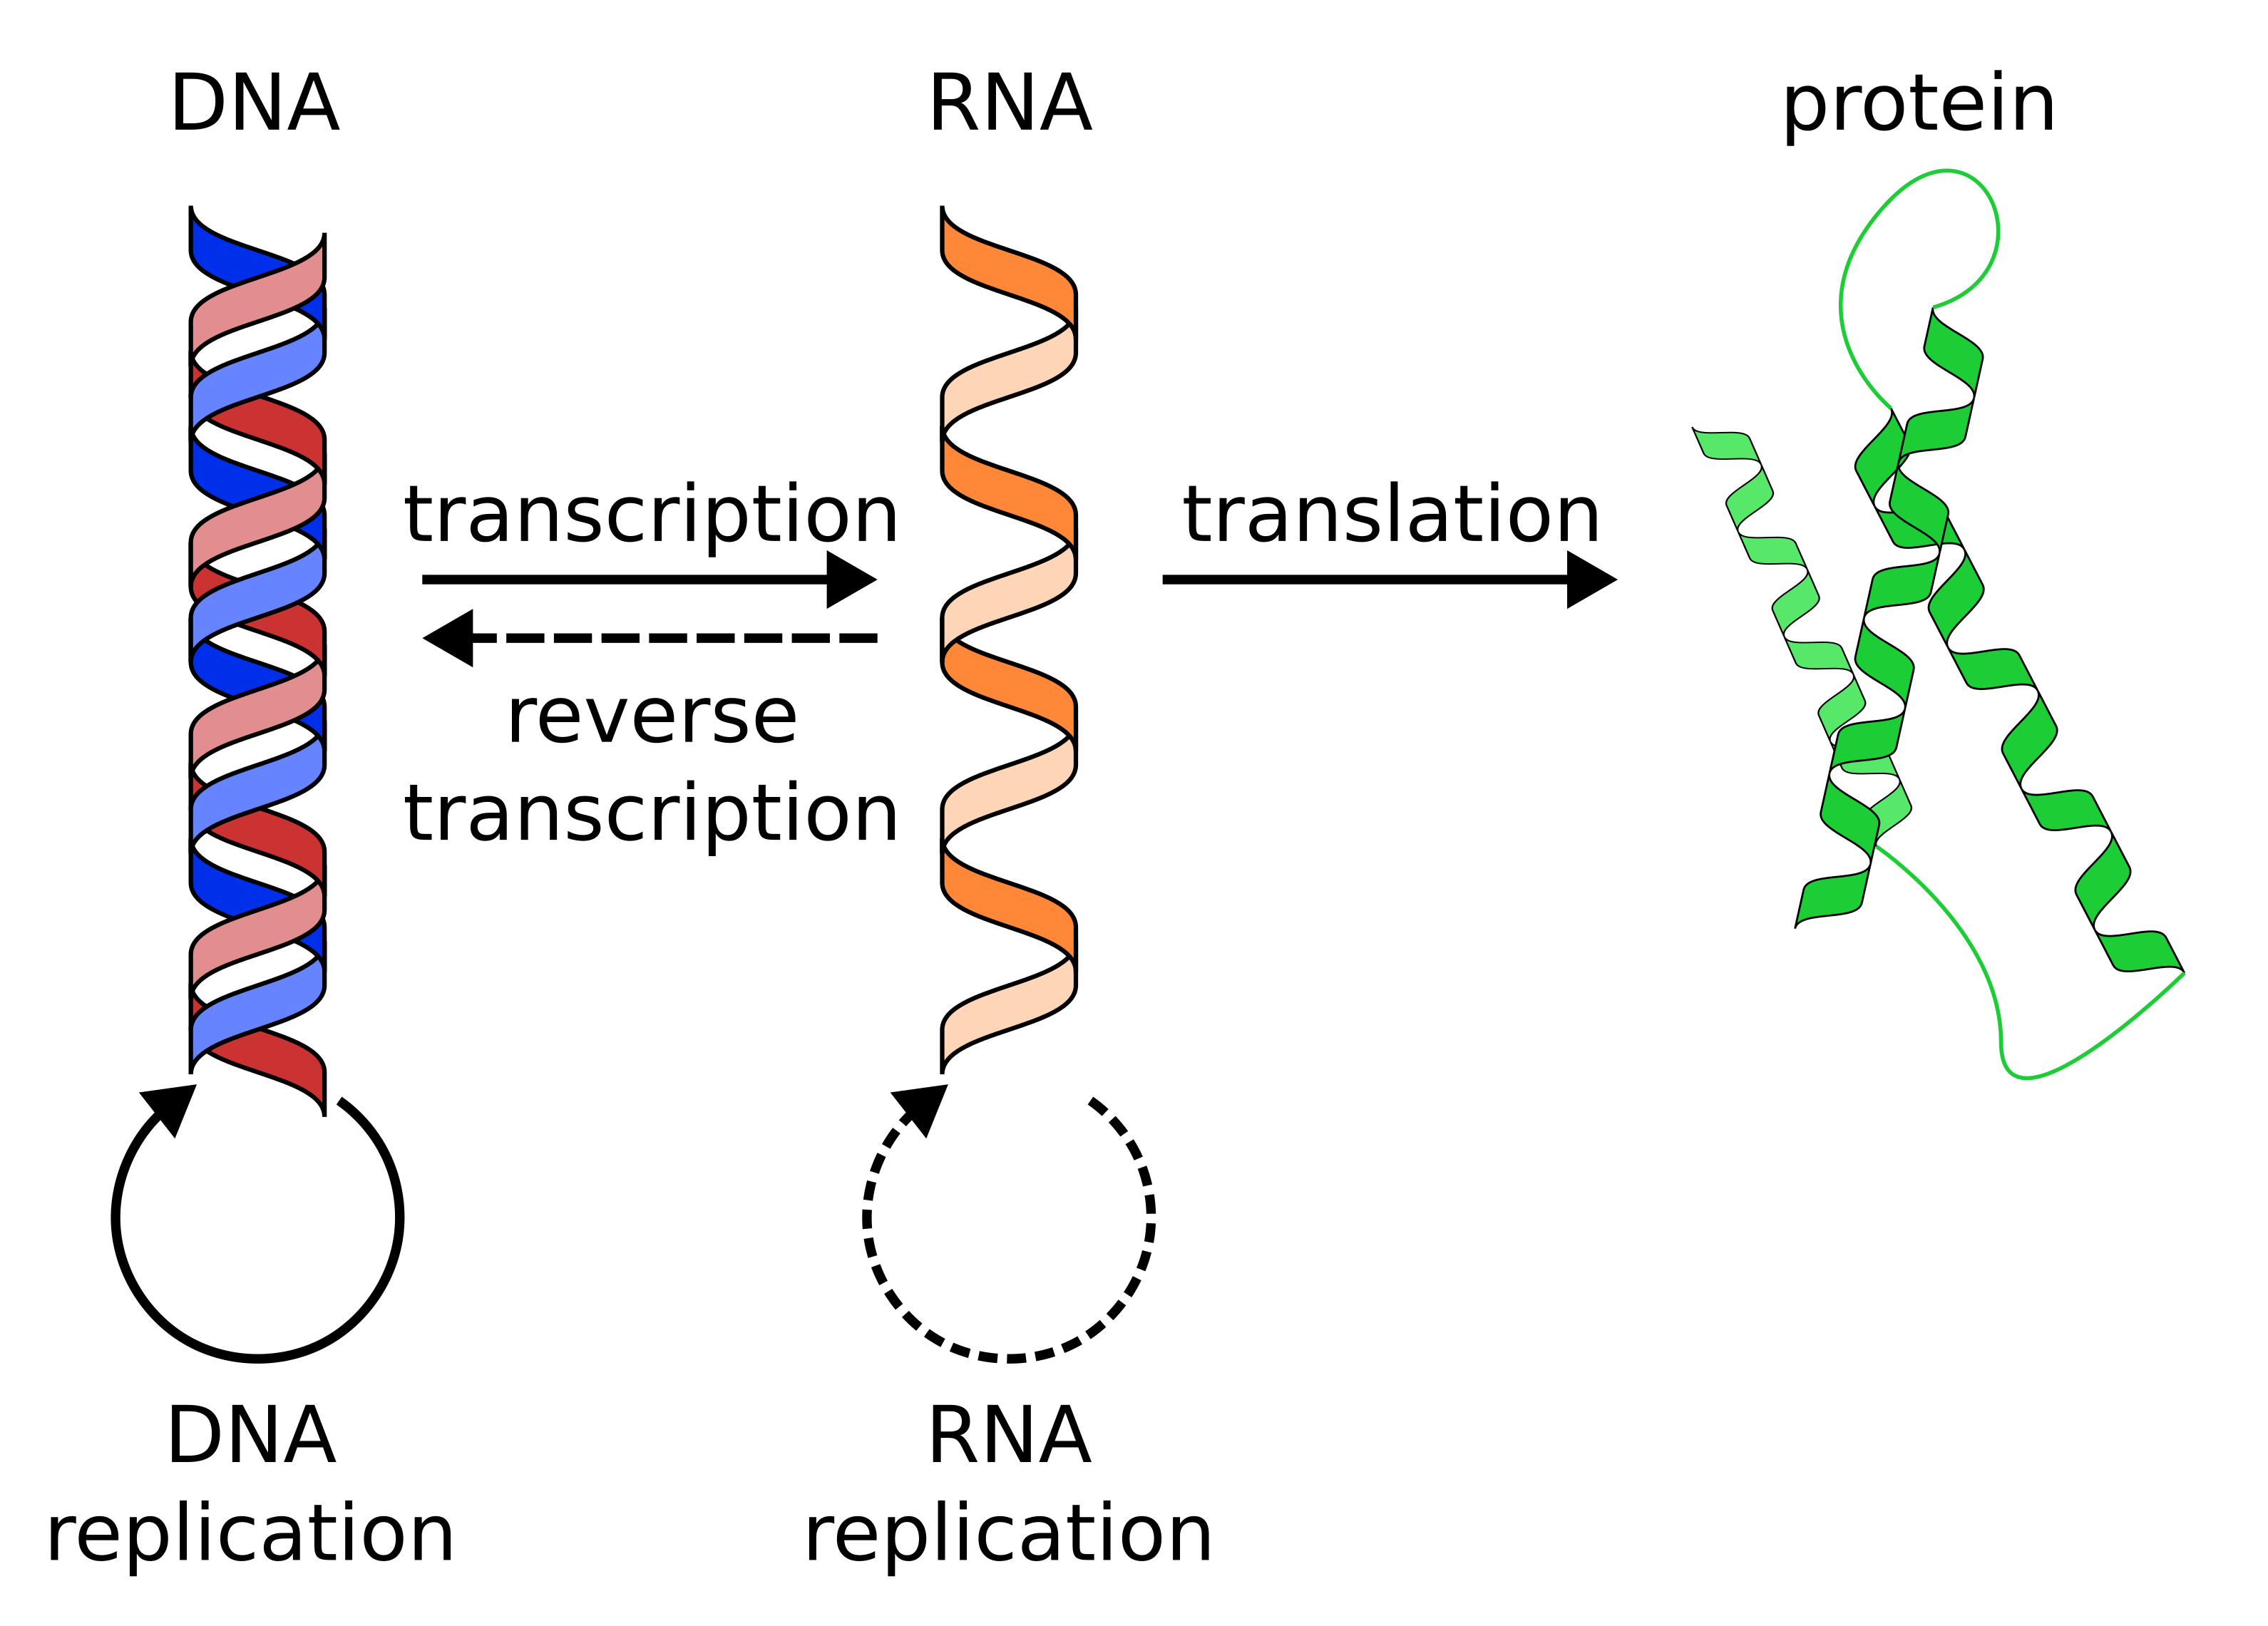
\includegraphics[width=\linewidth]{ch.introduction/imgs/central_dogma.png}
    \caption{\textbf{The central dogma of molecular biology.} Solid arrows indicate the general flow of information in the system, and dotted arrows are special cases.}
    \label{fig:central_dogma}
\end{figure}

The central dogma of molecular biology describes the flow of genetic information within a biological system. Whereas in a computer information is stored in bits, which can be either zero (0) or one (1), genetic information is stored in nucleotides, which can be either adenine (A), cytosine (C), guanine (G), or thymine (T). DNA, which stands for deoxyribonucleic acid, is composed of two large strands of these nucleotides that together form a double helix. Both strands contain the same information, but where there is a nucleotide A on one strand, there is always a corresponding nucleotide T on the other, and similarly for C and G. RNA, on the other hand, is a similar molecule but is typically single-stranded. It is transcribed from DNA and shares a similar nucleotide composition but replaces thymine (T) with uracil (U). RNA serves as the bridge between DNA and proteins. Through the process of translation, the information encoded in RNA is decoded and used to assemble chains of amino acids, ultimately resulting in the synthesis of proteins. Proteins carry out various tasks in our bodies, such as enabling chemical reactions, transporting other molecules, providing structure, and acting as regulators of transcription and translation of genes.

Far from all the DNA is transcribed into RNA, and not even all RNA translates to protein. As a general rule of thumb, we distinguish DNA sequences that get transcribed into RNA as genes. The human genome consists of approximately 20.000 genes, and the coding parts of these genes represent approximately 6\% of the genome\cite{Piovesan2019}. Early molecular biologists mainly focused on coding genes, thus the remaining 94\% got known as ``junk DNA''. We now know, however, that at least 80\% of human DNA is involved in at least one biochemical function\cite{encode2012}. Almost all of these functions are related to gene expression regulation.

% \subsection{Transcription}

% \begin{figure}[hbtp]
%     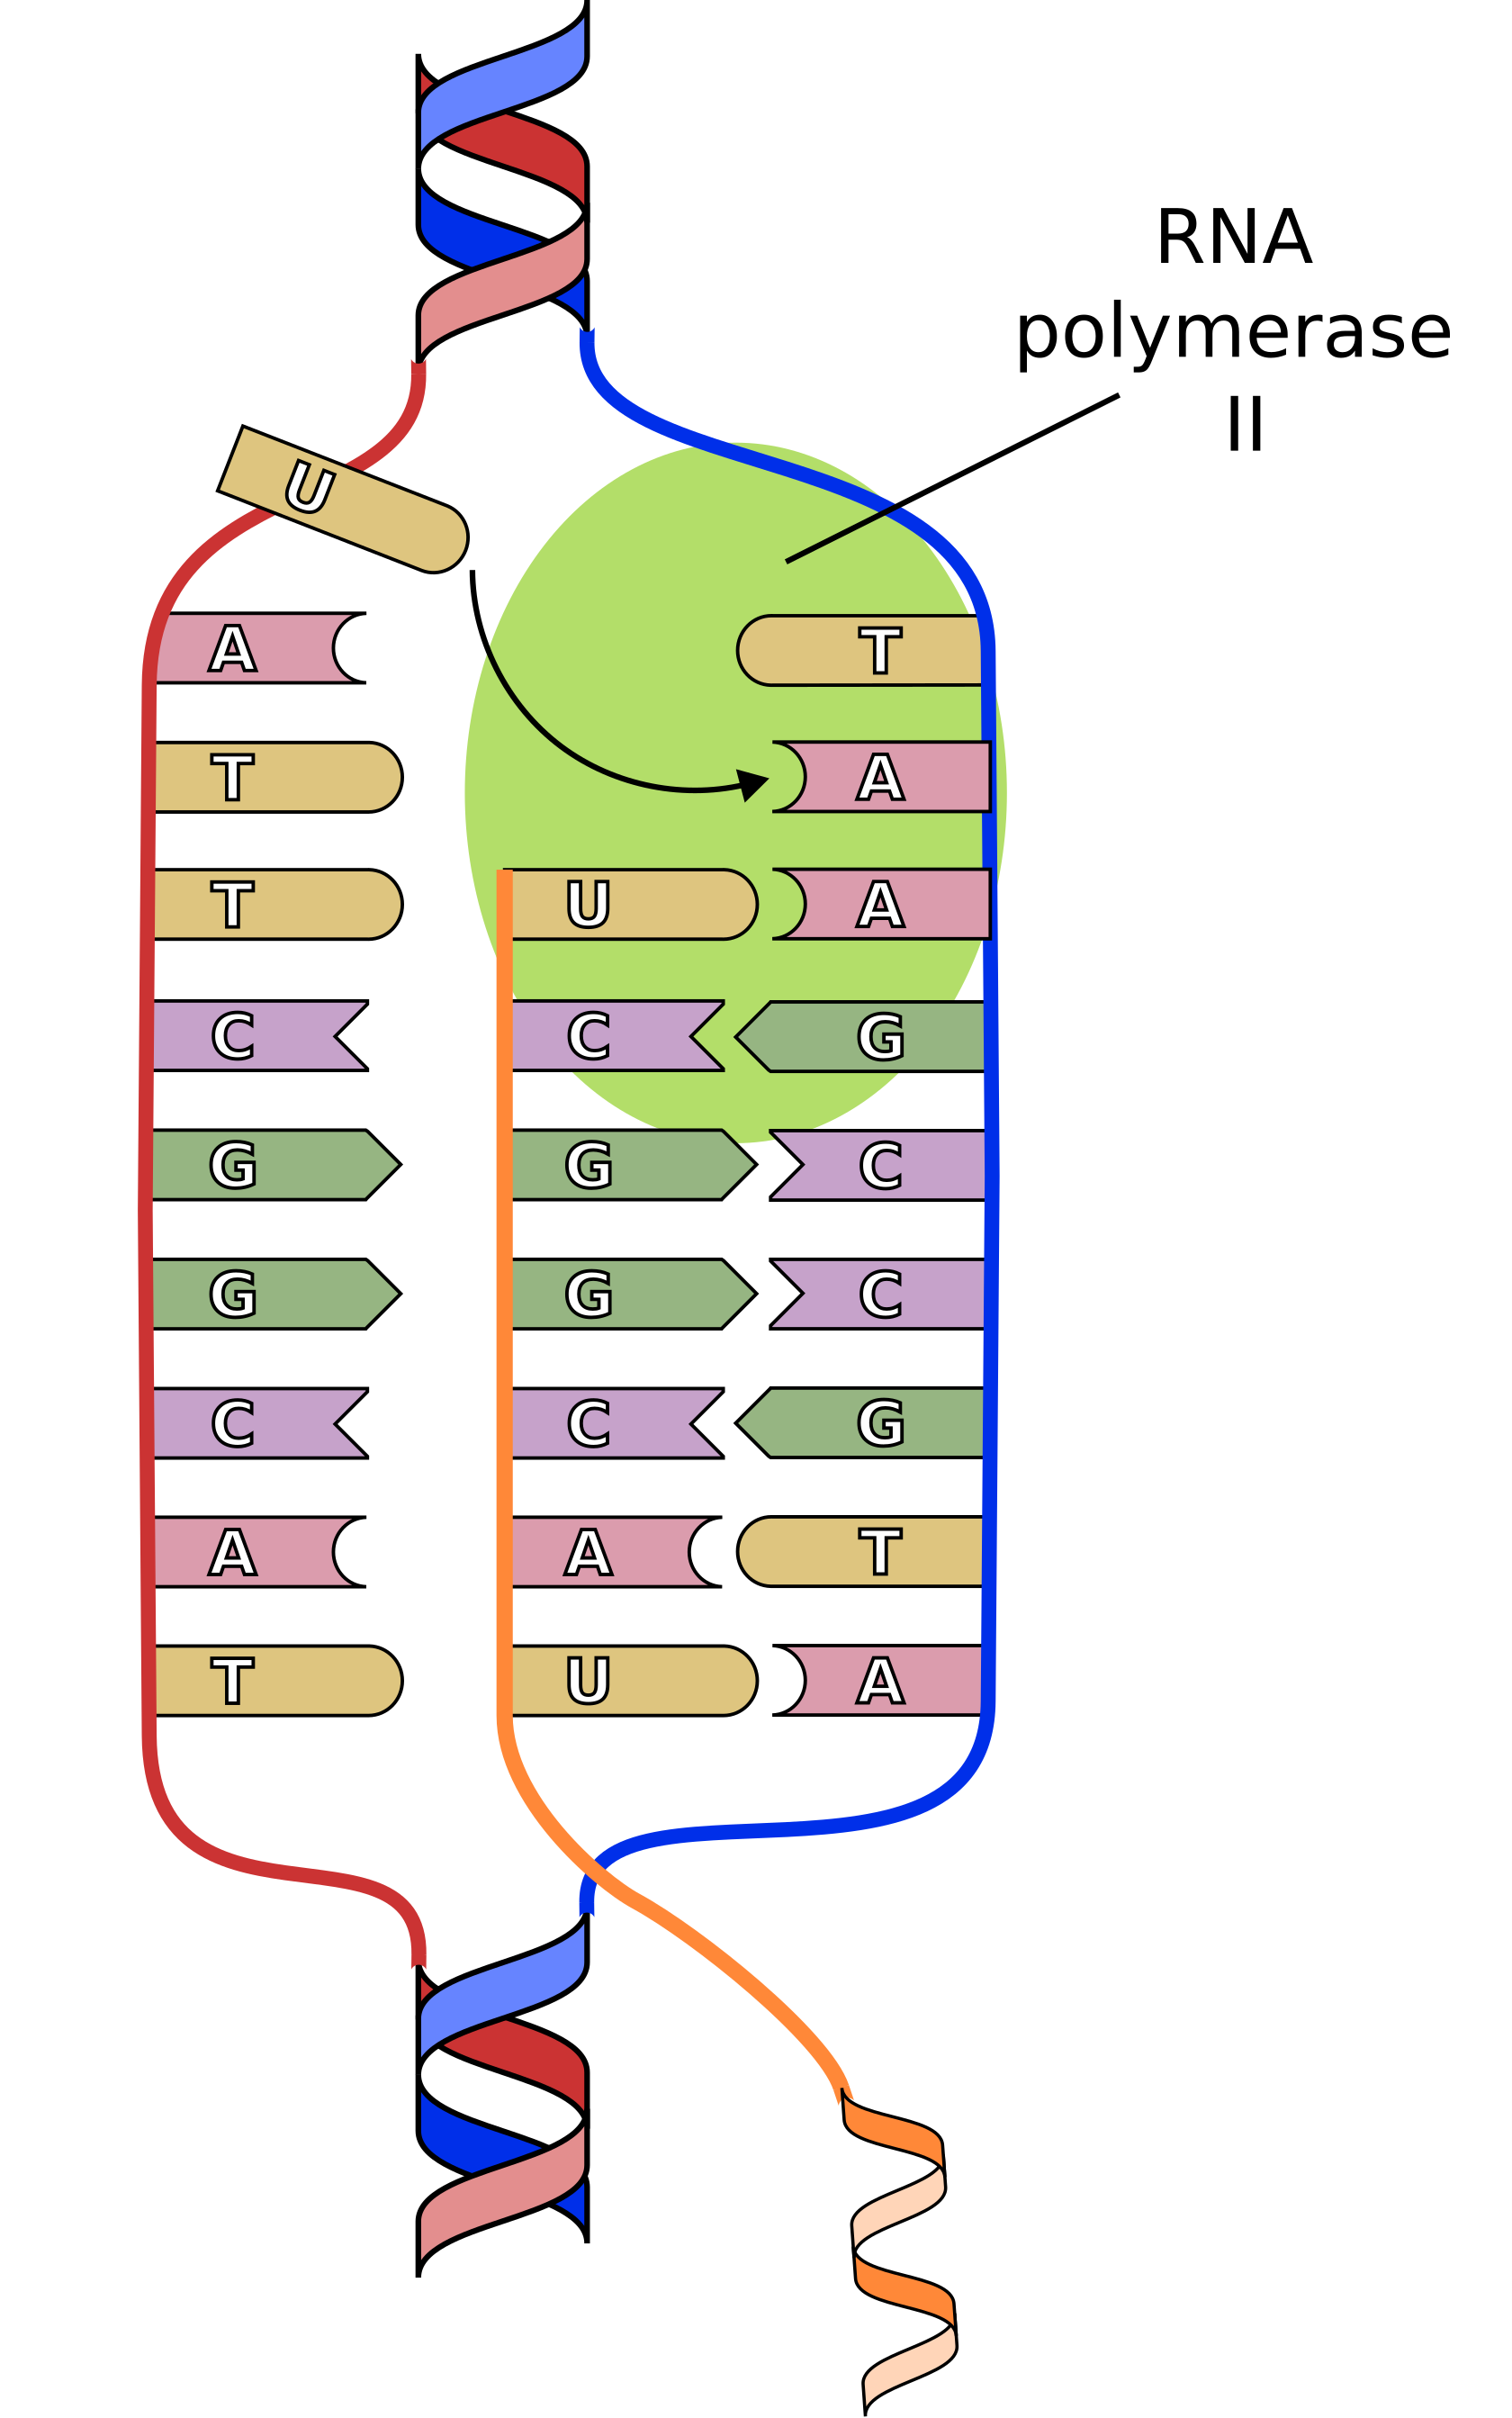
\includegraphics[height=0.5\textheight]{ch.introduction/imgs/transcription.png}
%     \caption{Caption}
%     \label{fig:transcription}
% \end{figure}

% \subsection{Translation}

% \begin{figure}[H]
%     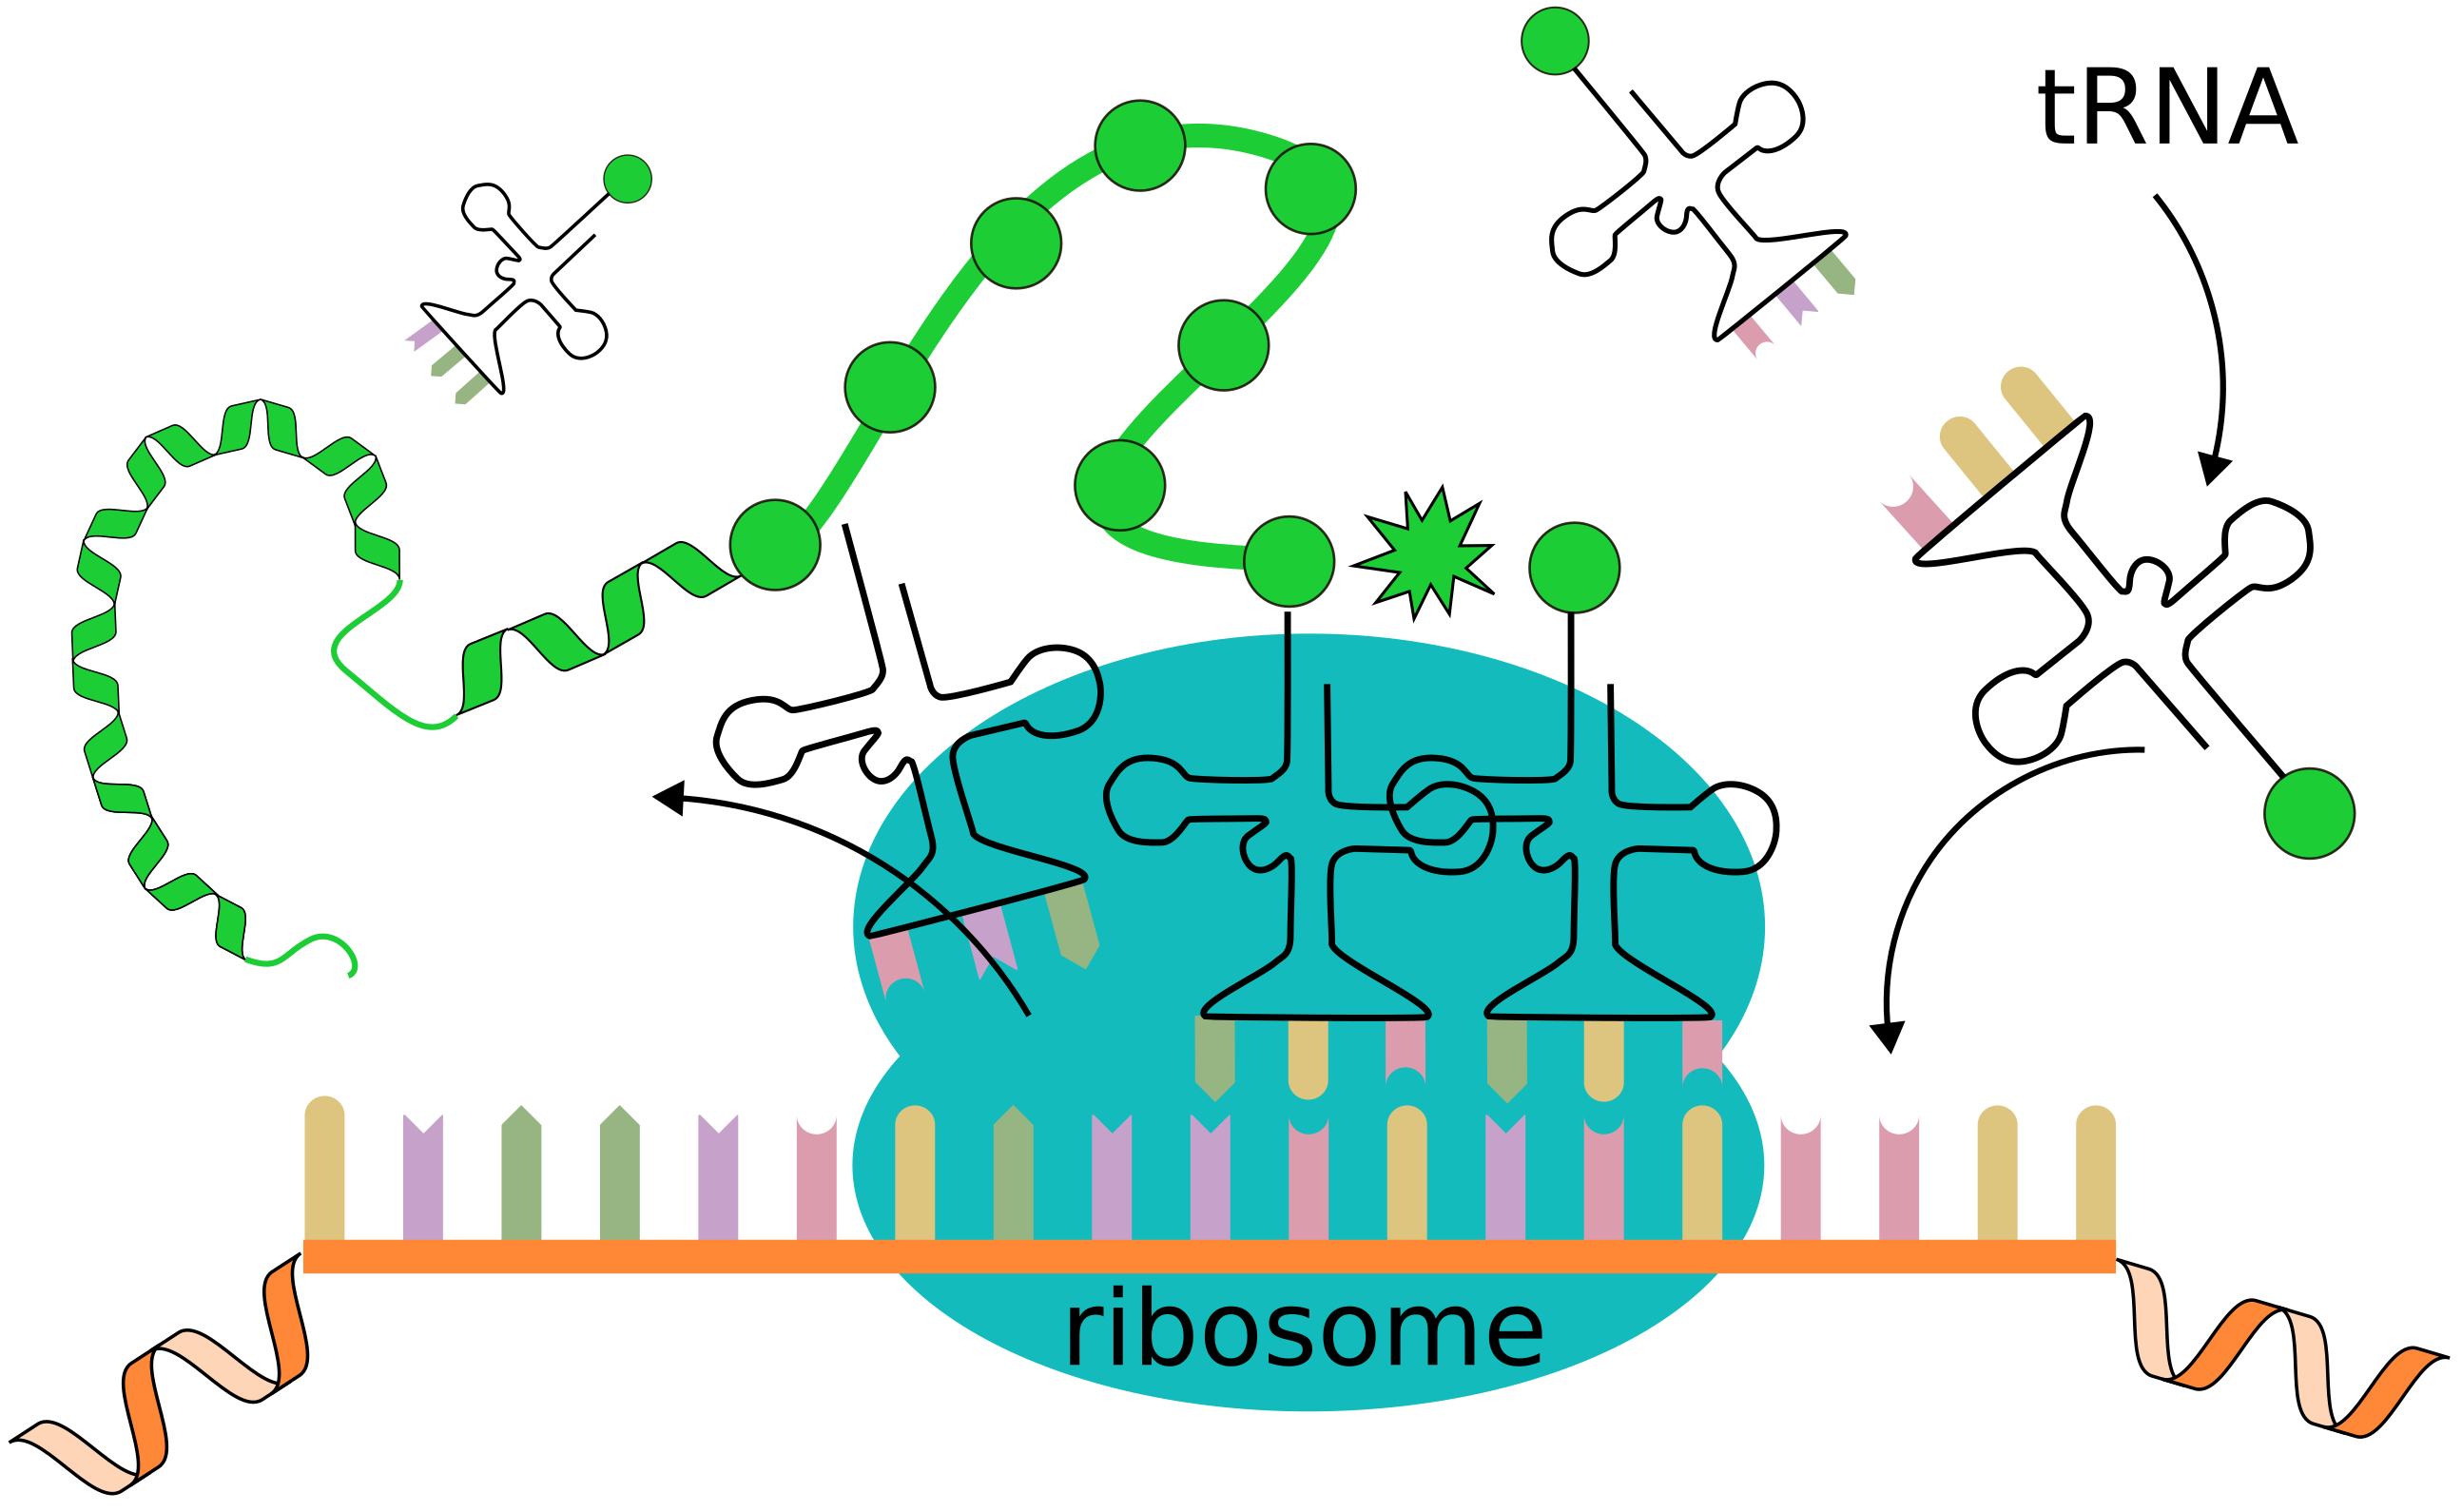
\includegraphics[width=\linewidth]{ch.introduction/imgs/translation.png}
%     \caption{Caption}
%     \label{fig:translation}
% \end{figure}

\section{Gene expression regulation}

A skin cell makes use of a completely different set of genes than a liver cell, even though they contain the same DNA. This is possible due to the tight regulation of gene expression by these cells. To regulate their gene expression cells have a wide array of tools at their disposal. 

\subsection{Transcription Factors}

At the start of each gene sits a promoter (fig. \ref{fig:TF}A). At the promoter general transcription factors bind, which in turn recruit RNA polymerase II (RNAPII). RNAPII is the protein complex responsible for transription, and in turn 

Before DNA transcription can occur, 

DNA transcription requires a wide array of steps. Slightly upstream of a gene is a promoter. To this piece of DNA proteins bind that initiate transcription.

motifs needed

\begin{figure}[H]
    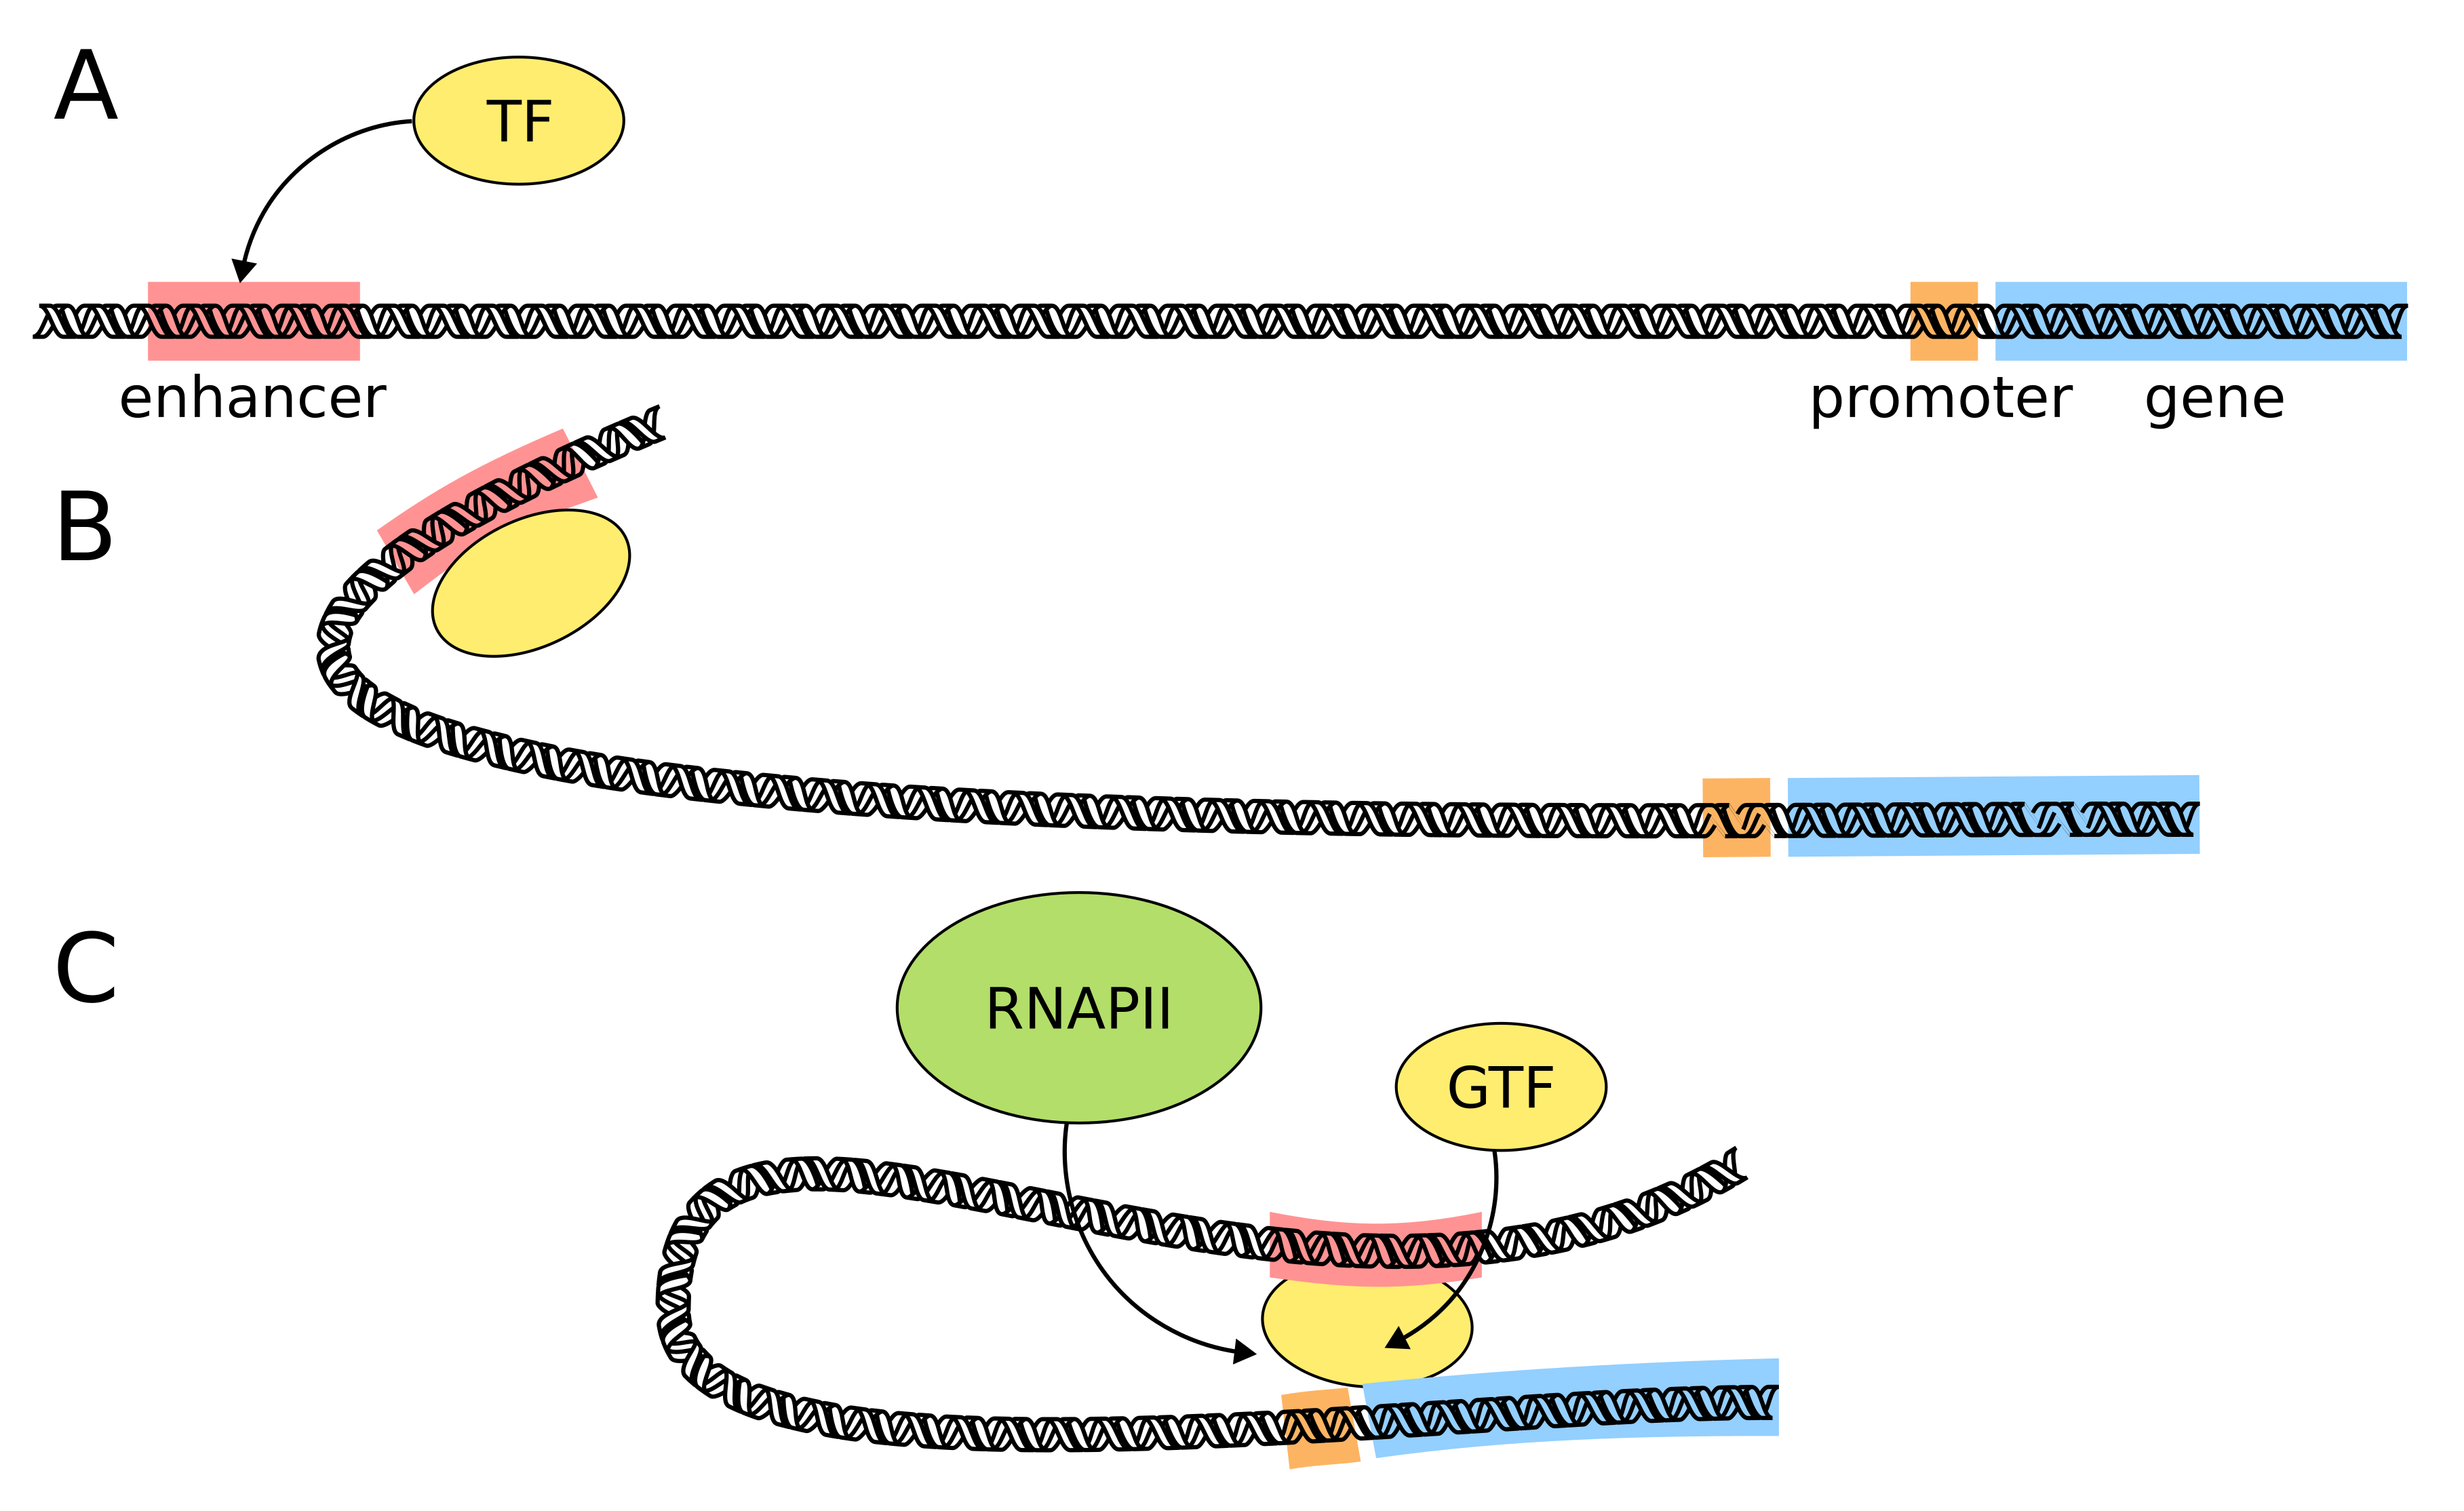
\includegraphics[width=\linewidth]{ch.introduction/imgs/transcription_factor.png}
    \caption{Caption}
    \label{fig:TF}
\end{figure}

\subsection{Chromatin context}

To fit 2 meters of DNA fold it

\begin{figure}[H]
    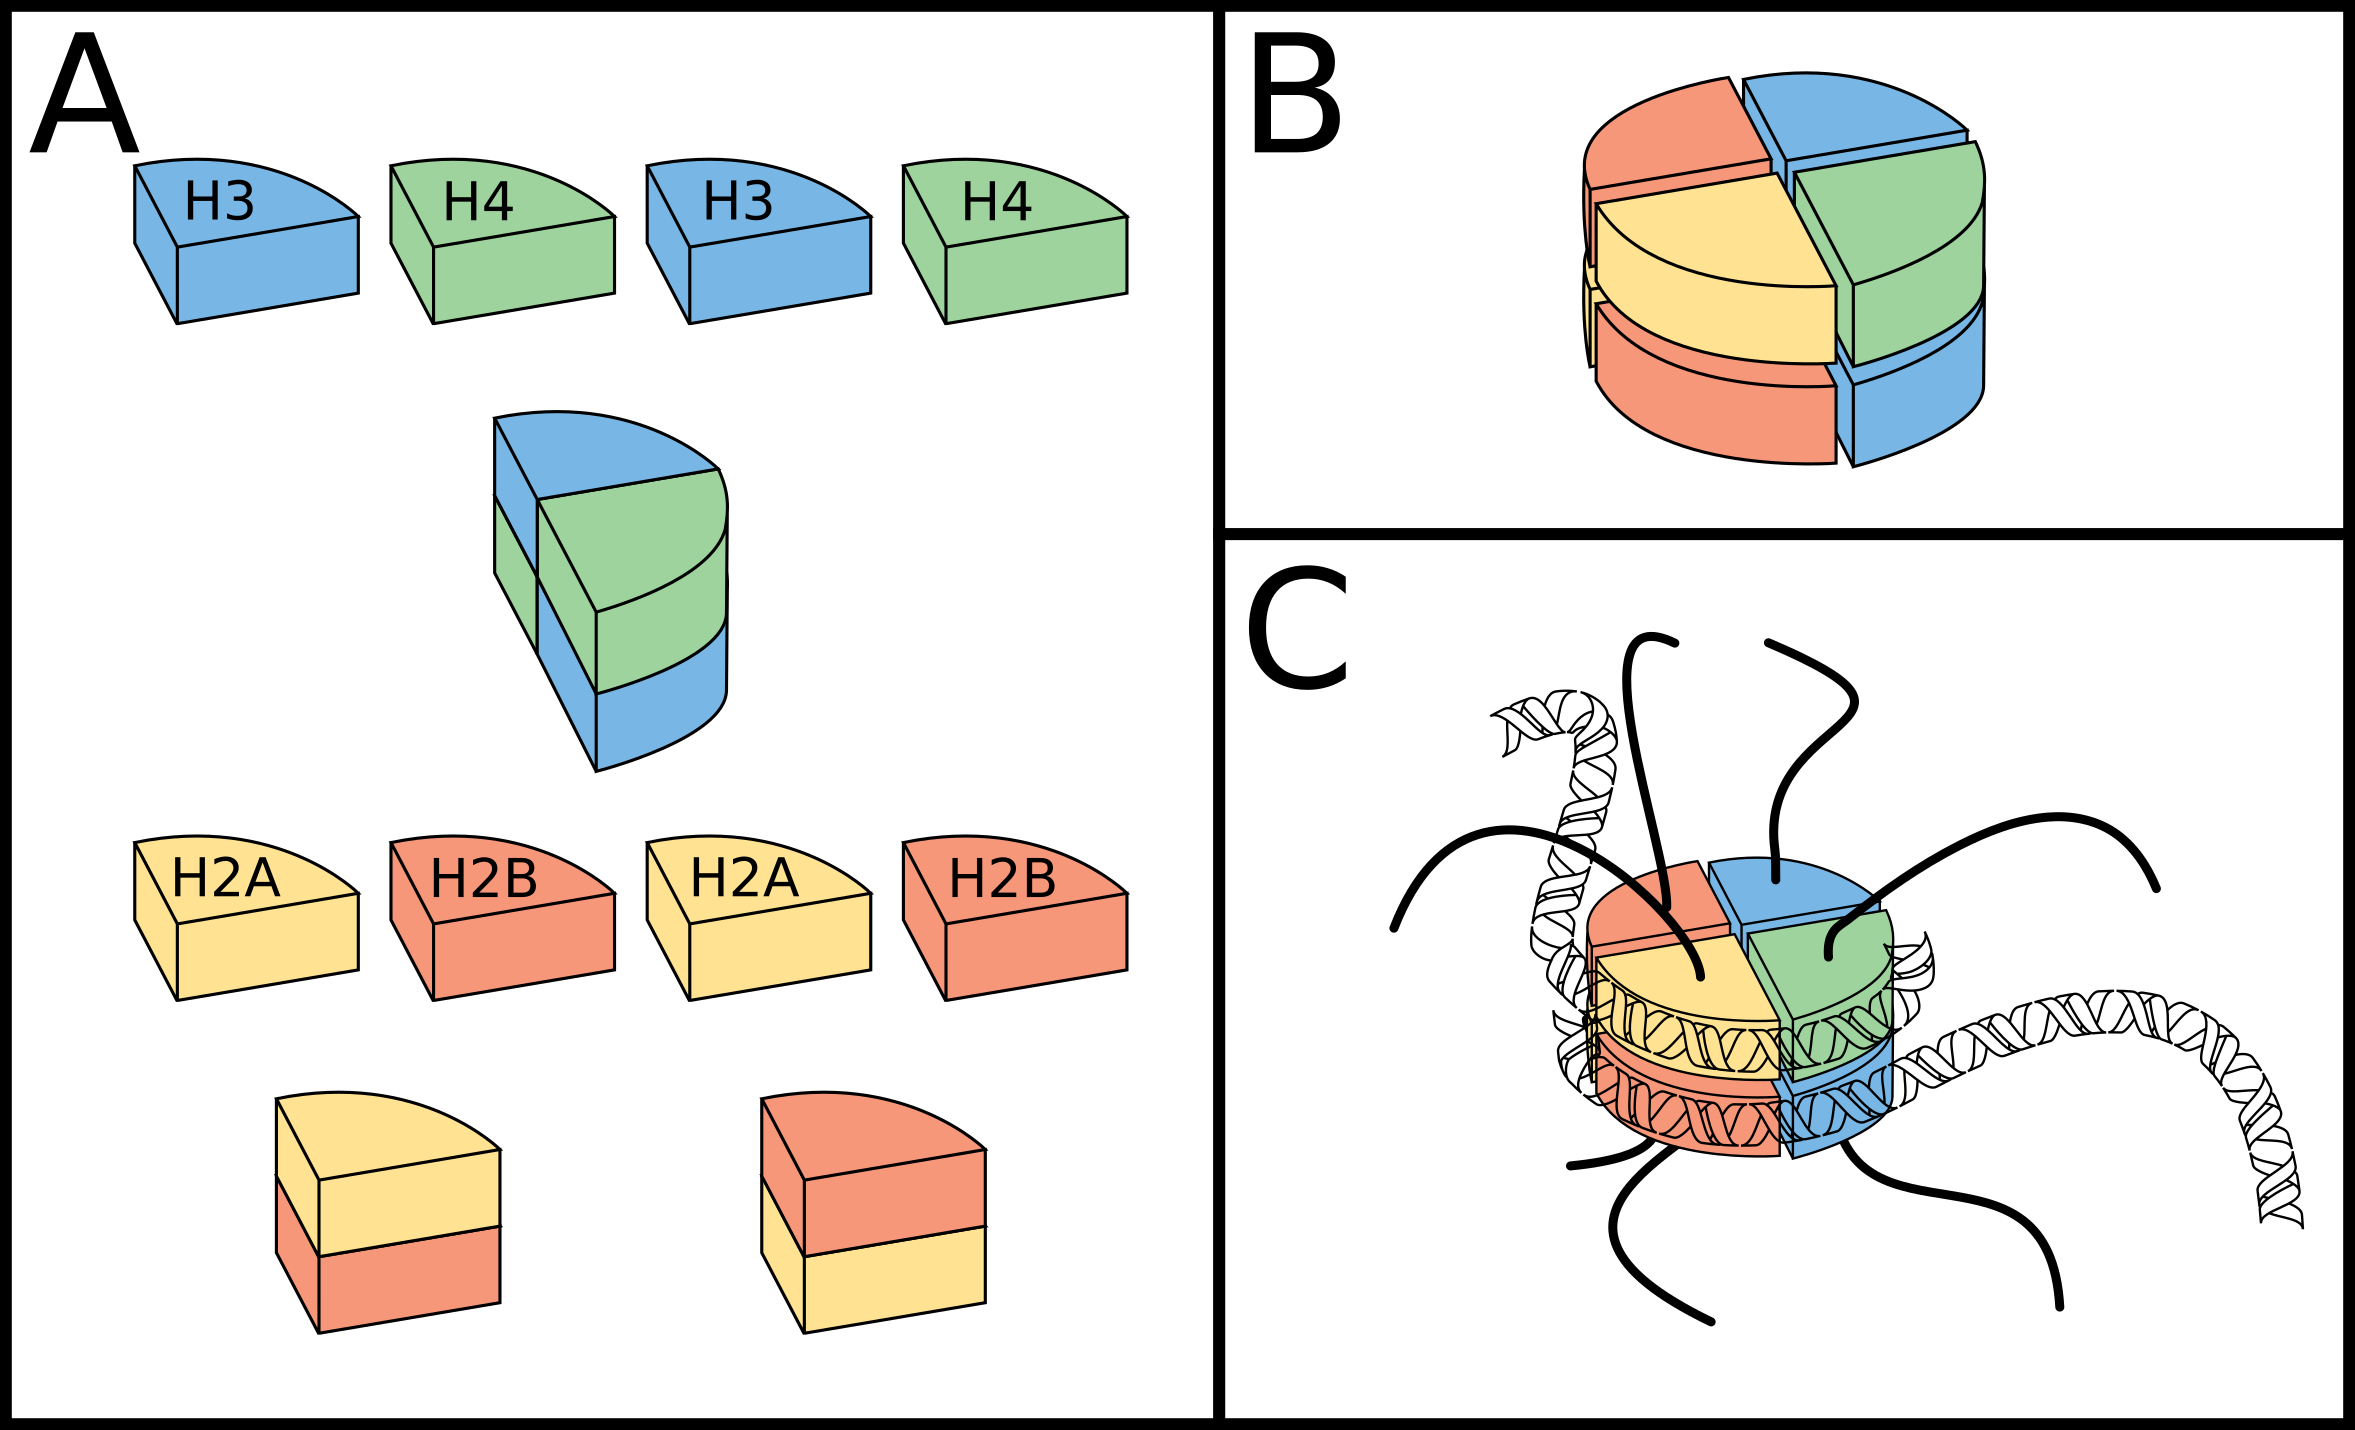
\includegraphics[width=\linewidth]{ch.introduction/imgs/histones.png}
    \caption{Caption}
    \label{fig:histones}
\end{figure}

\begin{figure}[H]
    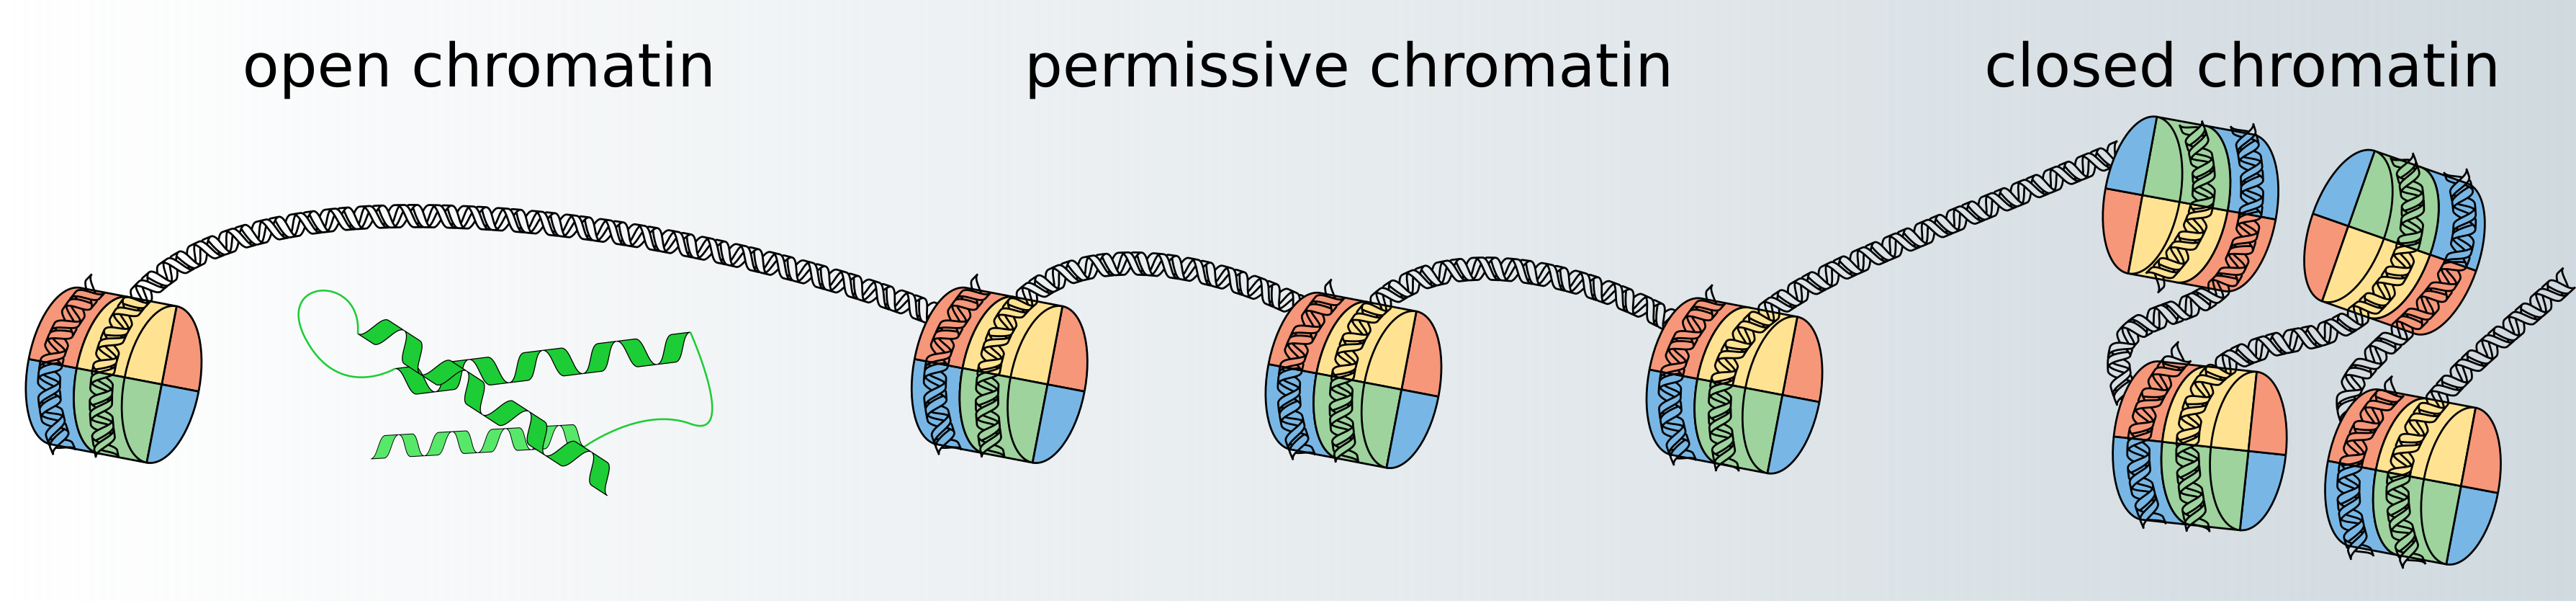
\includegraphics[width=\linewidth]{ch.introduction/imgs/accessibility_horizontal.png}
    \caption{Caption}
    \label{fig:accessibility}
\end{figure}

\hvFloat[doublePage,capWidth=n,
capPos=right,capVPos=top,bindCorr=0.0cm]{figure}
{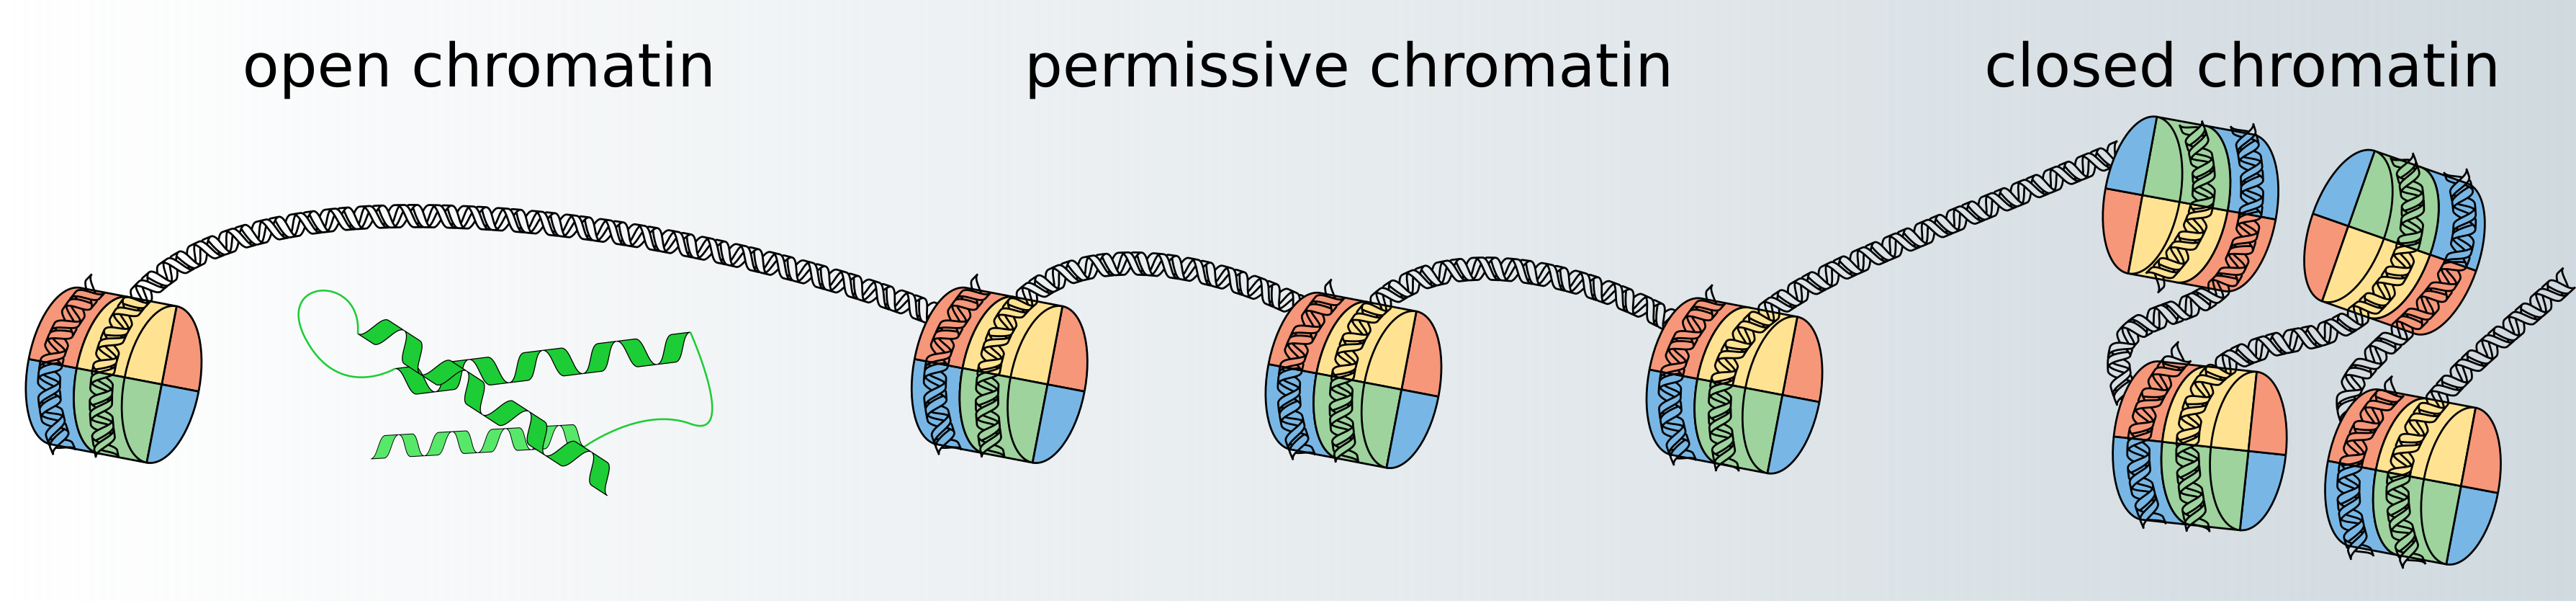
\includegraphics[width=1.6\textwidth]
{ch.introduction/imgs/accessibility_horizontal.png}}
[accessibility schematic overview]
{DNA accessibility regulates whether proteins can bind or not. Lorum ipsum lor Lorum ipsum lor Lorum ipsum lor Lorum ipsum lor Lorum ipsum lor Lorum ipsum lor Lorum ipsum lor Lorum ipsum lor}{fig:accessibility}
% \hvFloat[doublePage,sameHeight]%
%     {figure}%
%     {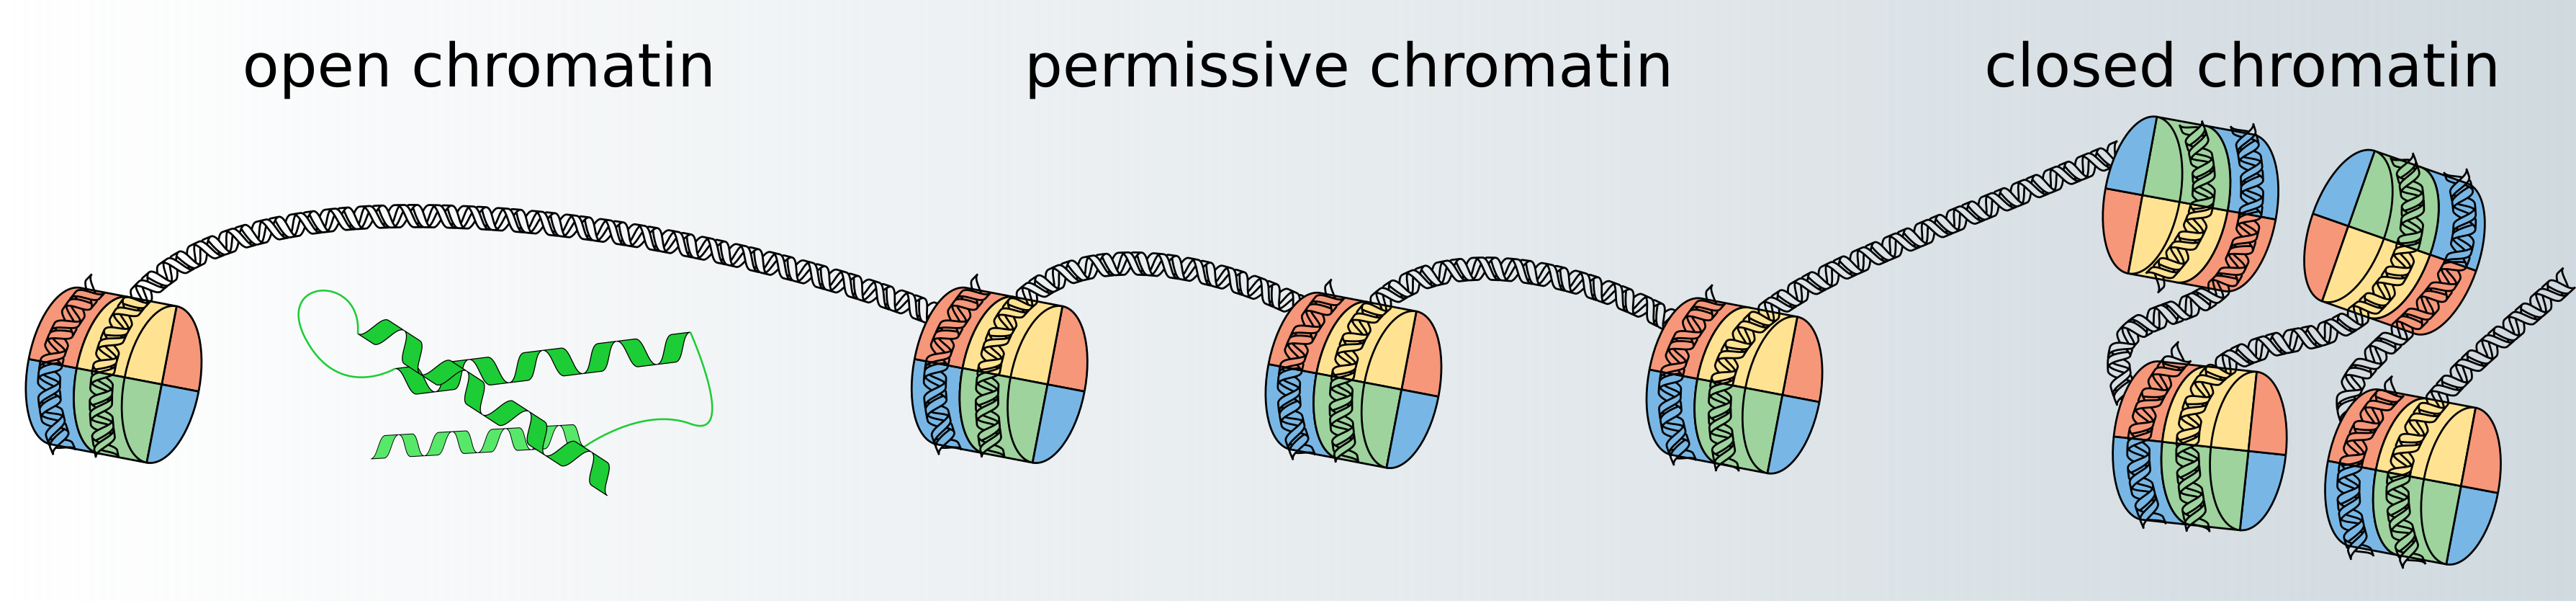
\includegraphics[doublefullPage]{ch.introduction/imgs/accessibility_horizontal.png}}%
%     [A doublepage image with a caption on the right side of the right part.]%
%     {A caption for a double-sided image that will be placed on the right side of the
%     right-hand part of the illustration. The illustration begins on the left edge of
%     the paper. A short form is used for the LOF.
%     The parameter is \texttt{doublePage}}%
    {fig:doublePage0sH}

\subsection{Other gene regulatory modes}
% \subsubsection{mRNA degradation}
% \subsubsection{Post-transcriptional modification}
% \subsubsection{RNA transport}
% \subsubsection{Signal transduction}

\subsection{Gene regulatory networks}

Mapping the relationship between genes is crucial for understanding how cellular processes are regulated. A common abstraction to understand gene-gene interactions are gene regulatory networks.  

The first gene regulatory network was proposed by Roy Britten and Eric Davidson in 1969\cite{Britten_1969}. They observed that a biological system (i) responds to an external signal; (ii) then produces its own signal as a response; (iii) transmits its own signal to receptors that do not perceive the external signal; (iv) then respond to its own signal, and finally (v) produces a protein as a response. Without modern knowledge of gene regulation, they then correctly reverse-engineered what the minimum requirements are for such a system. One of the things they then predicted was the existence of transcription factors and promoter sequences. It took Eric Davidson more than 30 years to experimentally validate his original work\cite{Davidson_2002}.

Gene regulatory networks are often modeled and visualized with direct gene-gene interactions (fig. \ref{fig:network}A). This means for instance that the protein product of gene $\alpha$ directly regulates the protein product of gene $\beta$, ignoring all steps in between. Even though this is a gross oversimplification of gene-gene interactions, these simple models can already exhibit complex behavior. One of the older and well-known examples of this complex behavior are Turing patterns, discovered by the famous computer scientist Alan Turing\cite{Turing1952}. We consider a system of two genes, gene $\alpha$ and gene $\beta$, where gene $\alpha$ upregulates itself and gene $\beta$, but gene $\beta$ inhibits gene $\alpha$ (fig. \ref{fig:network}B). When modeling this simple two-gene network in a spatial setting it produces complex patterns (fig. \ref{fig:network}C), of which similar patterns can be observed in nature (fig. \ref{fig:network}D).

\begin{figure}[H]
    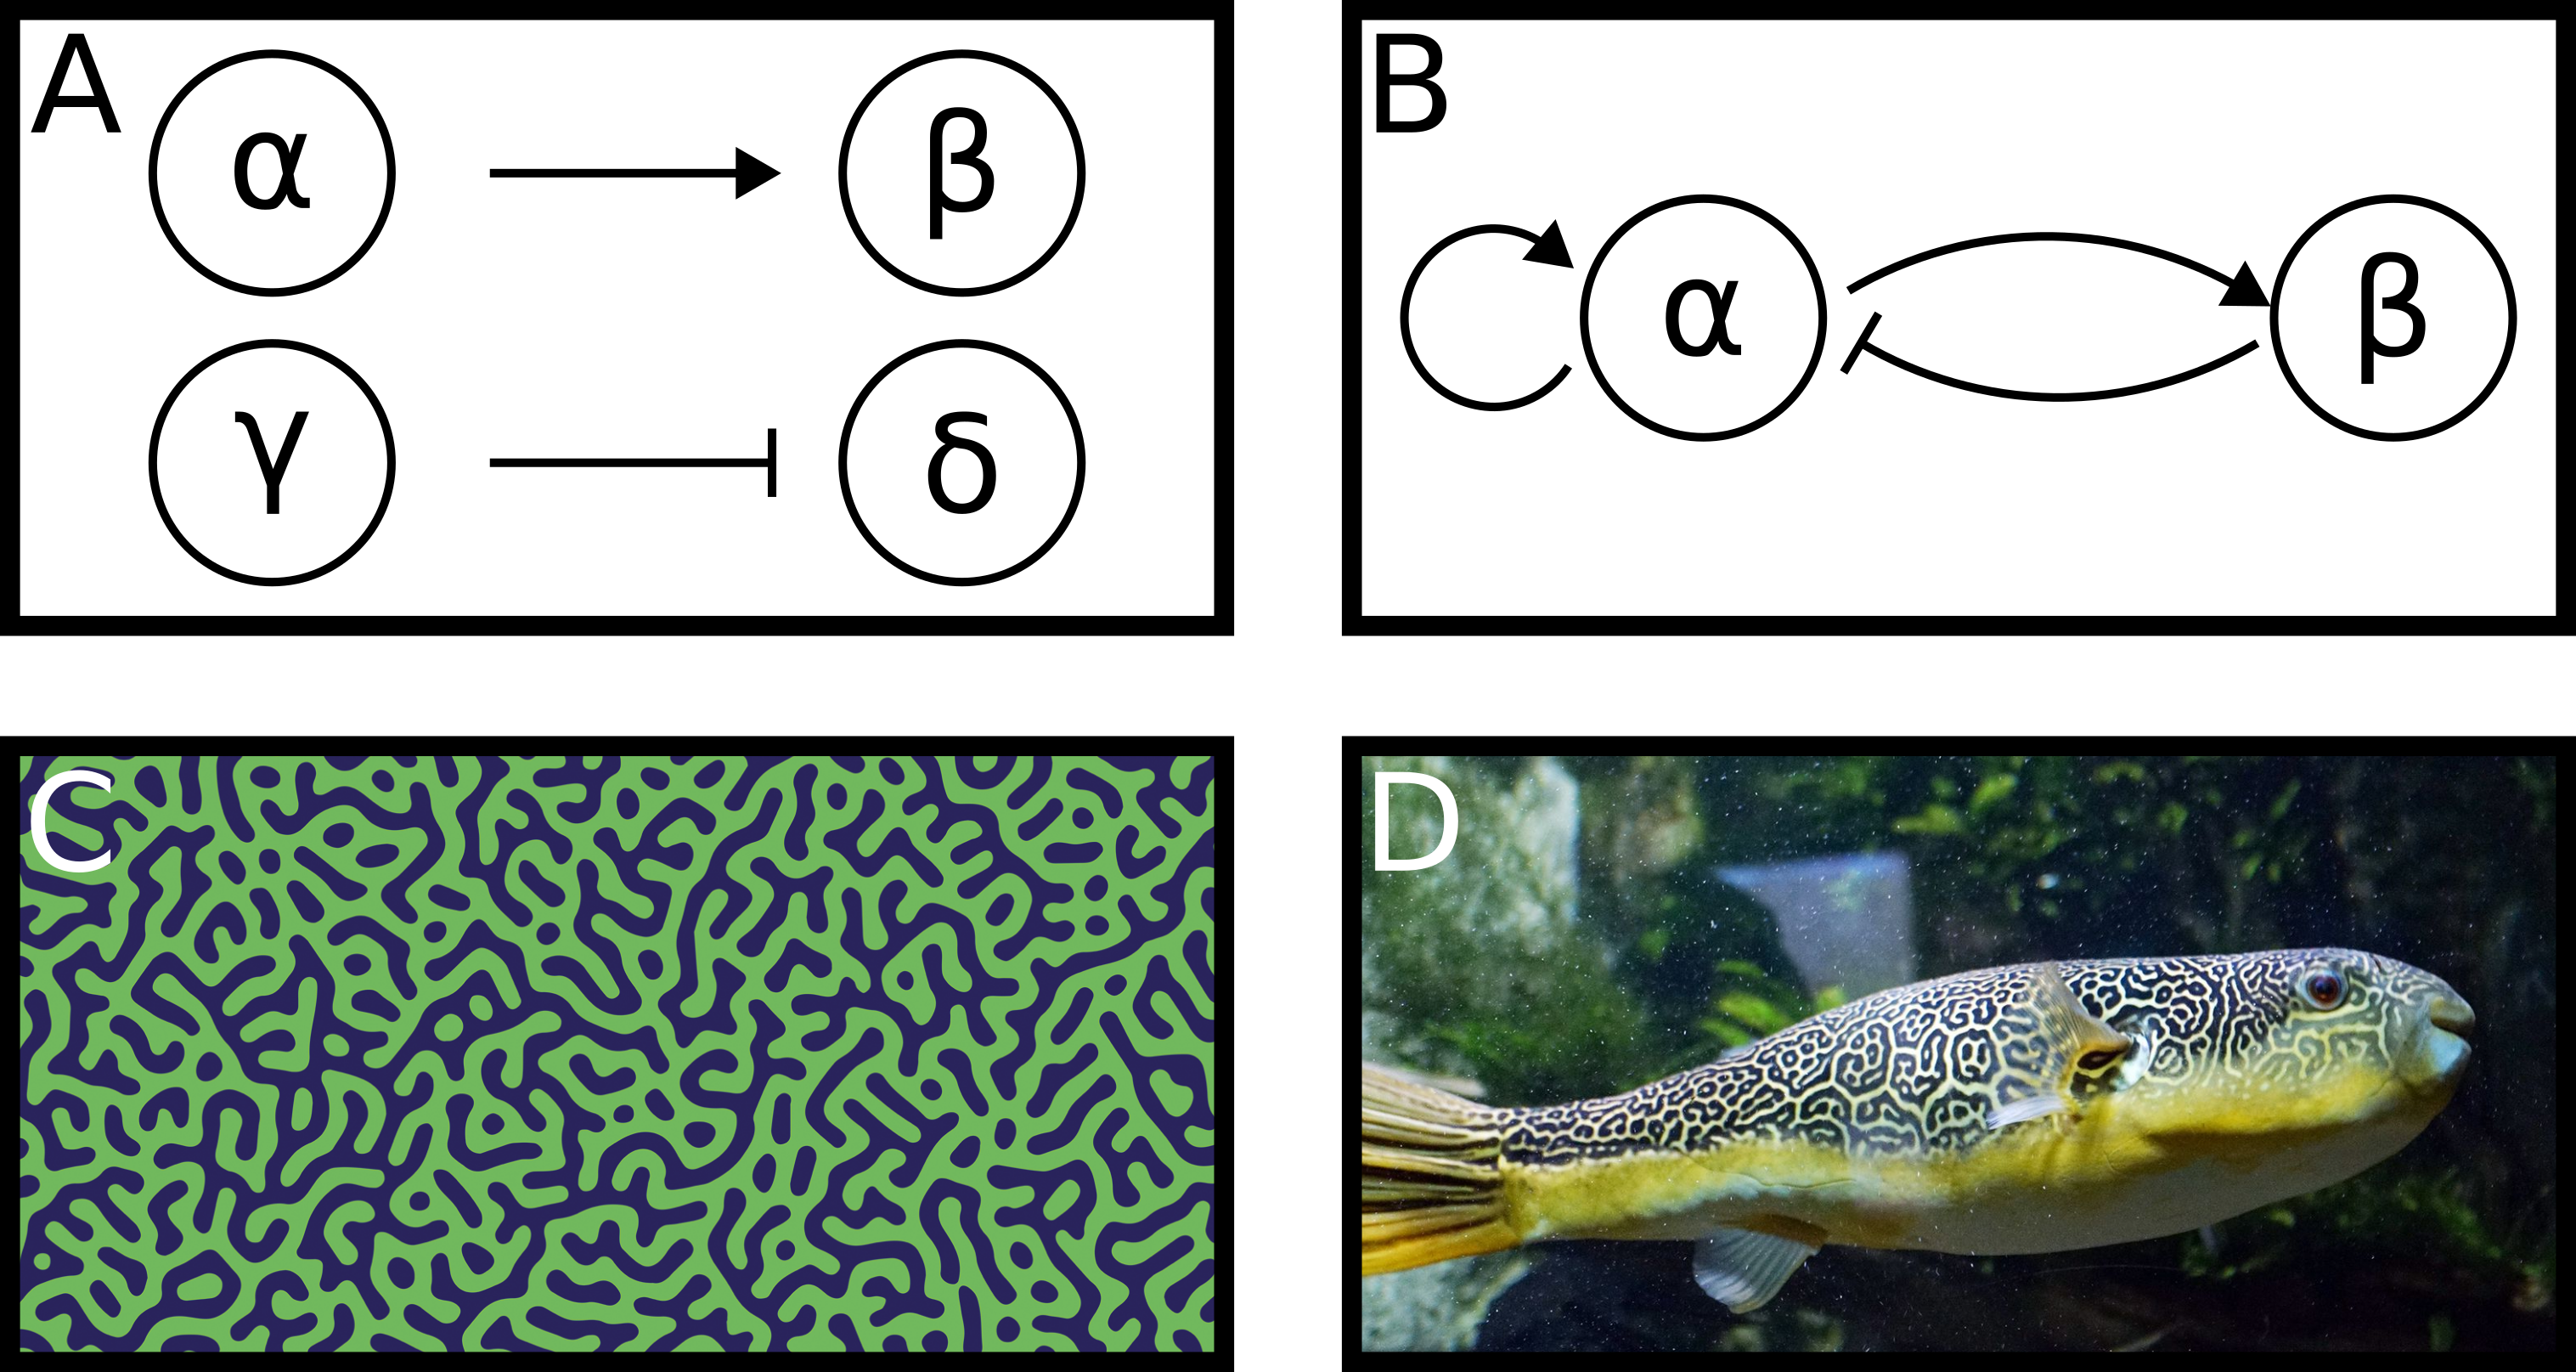
\includegraphics[width=\linewidth]{ch.introduction/imgs/network.png}
    \caption{(\textbf{A}) standard way of representing gene-gene interactions. Gene $\alpha$ upregulates gene $\beta$, and gene $\gamma$ downregulates gene $\delta$. (\textbf{B}) Gierer-Meinhardt gene regulatory network, where gene $\alpha$ upregulates itself and gene $\beta$, and gene $\beta$ downregulates gene $\alpha$. (\textbf{C}) Simulation of the Gierer-Meinhardt gene regulatory network in a spatial context. (\textbf{D}) A Mbuna pufferfish with Turing pattern. Image from Tiia Monto(https://en.wikipedia.org/wiki/Mbu\_pufferfish\#/media/File:Tetraodon\_mbu\_2.jpg)}
    \label{fig:network}
\end{figure}

TODO more recent / complex gene networks. 

\section{Evolutionary development (evo-devo)}

A single fertilized egg cell develops into a complex collection of trillions of cells by the time the individual reaches adulthood. How does each cell know what to develop into? In the 1980s scientists discovered a set of genes in fruit flies responsible for strange transformations. A mutation in one of these genes caused flies to grow legs instead of antennae from their mouths\cite{Schneuwly1987}, or it caused flies to develop a second pair of wings\cite{Weatherbee1998}. This work showed that antennae cells contain all the information necessary to build legs. This set of genes is now known as the HOX genes.

The development of fruit flies starts as worm-like creatures build up from multiple segments. Hox genes in different segments determine each segment's identity and guide its growth. For example, HOX genes in the head control mouth parts and antennae, while HOX genes in the thorax direct leg and wing development. Interestingly, the order of HOX genes on the chromosome is the same as the order in which they appear along the segments of the body. 

Nearly all animals have HOX genes.
  
% https://learn.genetics.utah.edu/content/basics/hoxgenes#:~:text=Fruit%20flies%20begin%20life%20as,what%20structures%20it%20should%20grow.

% \begin{figure}[H]
%     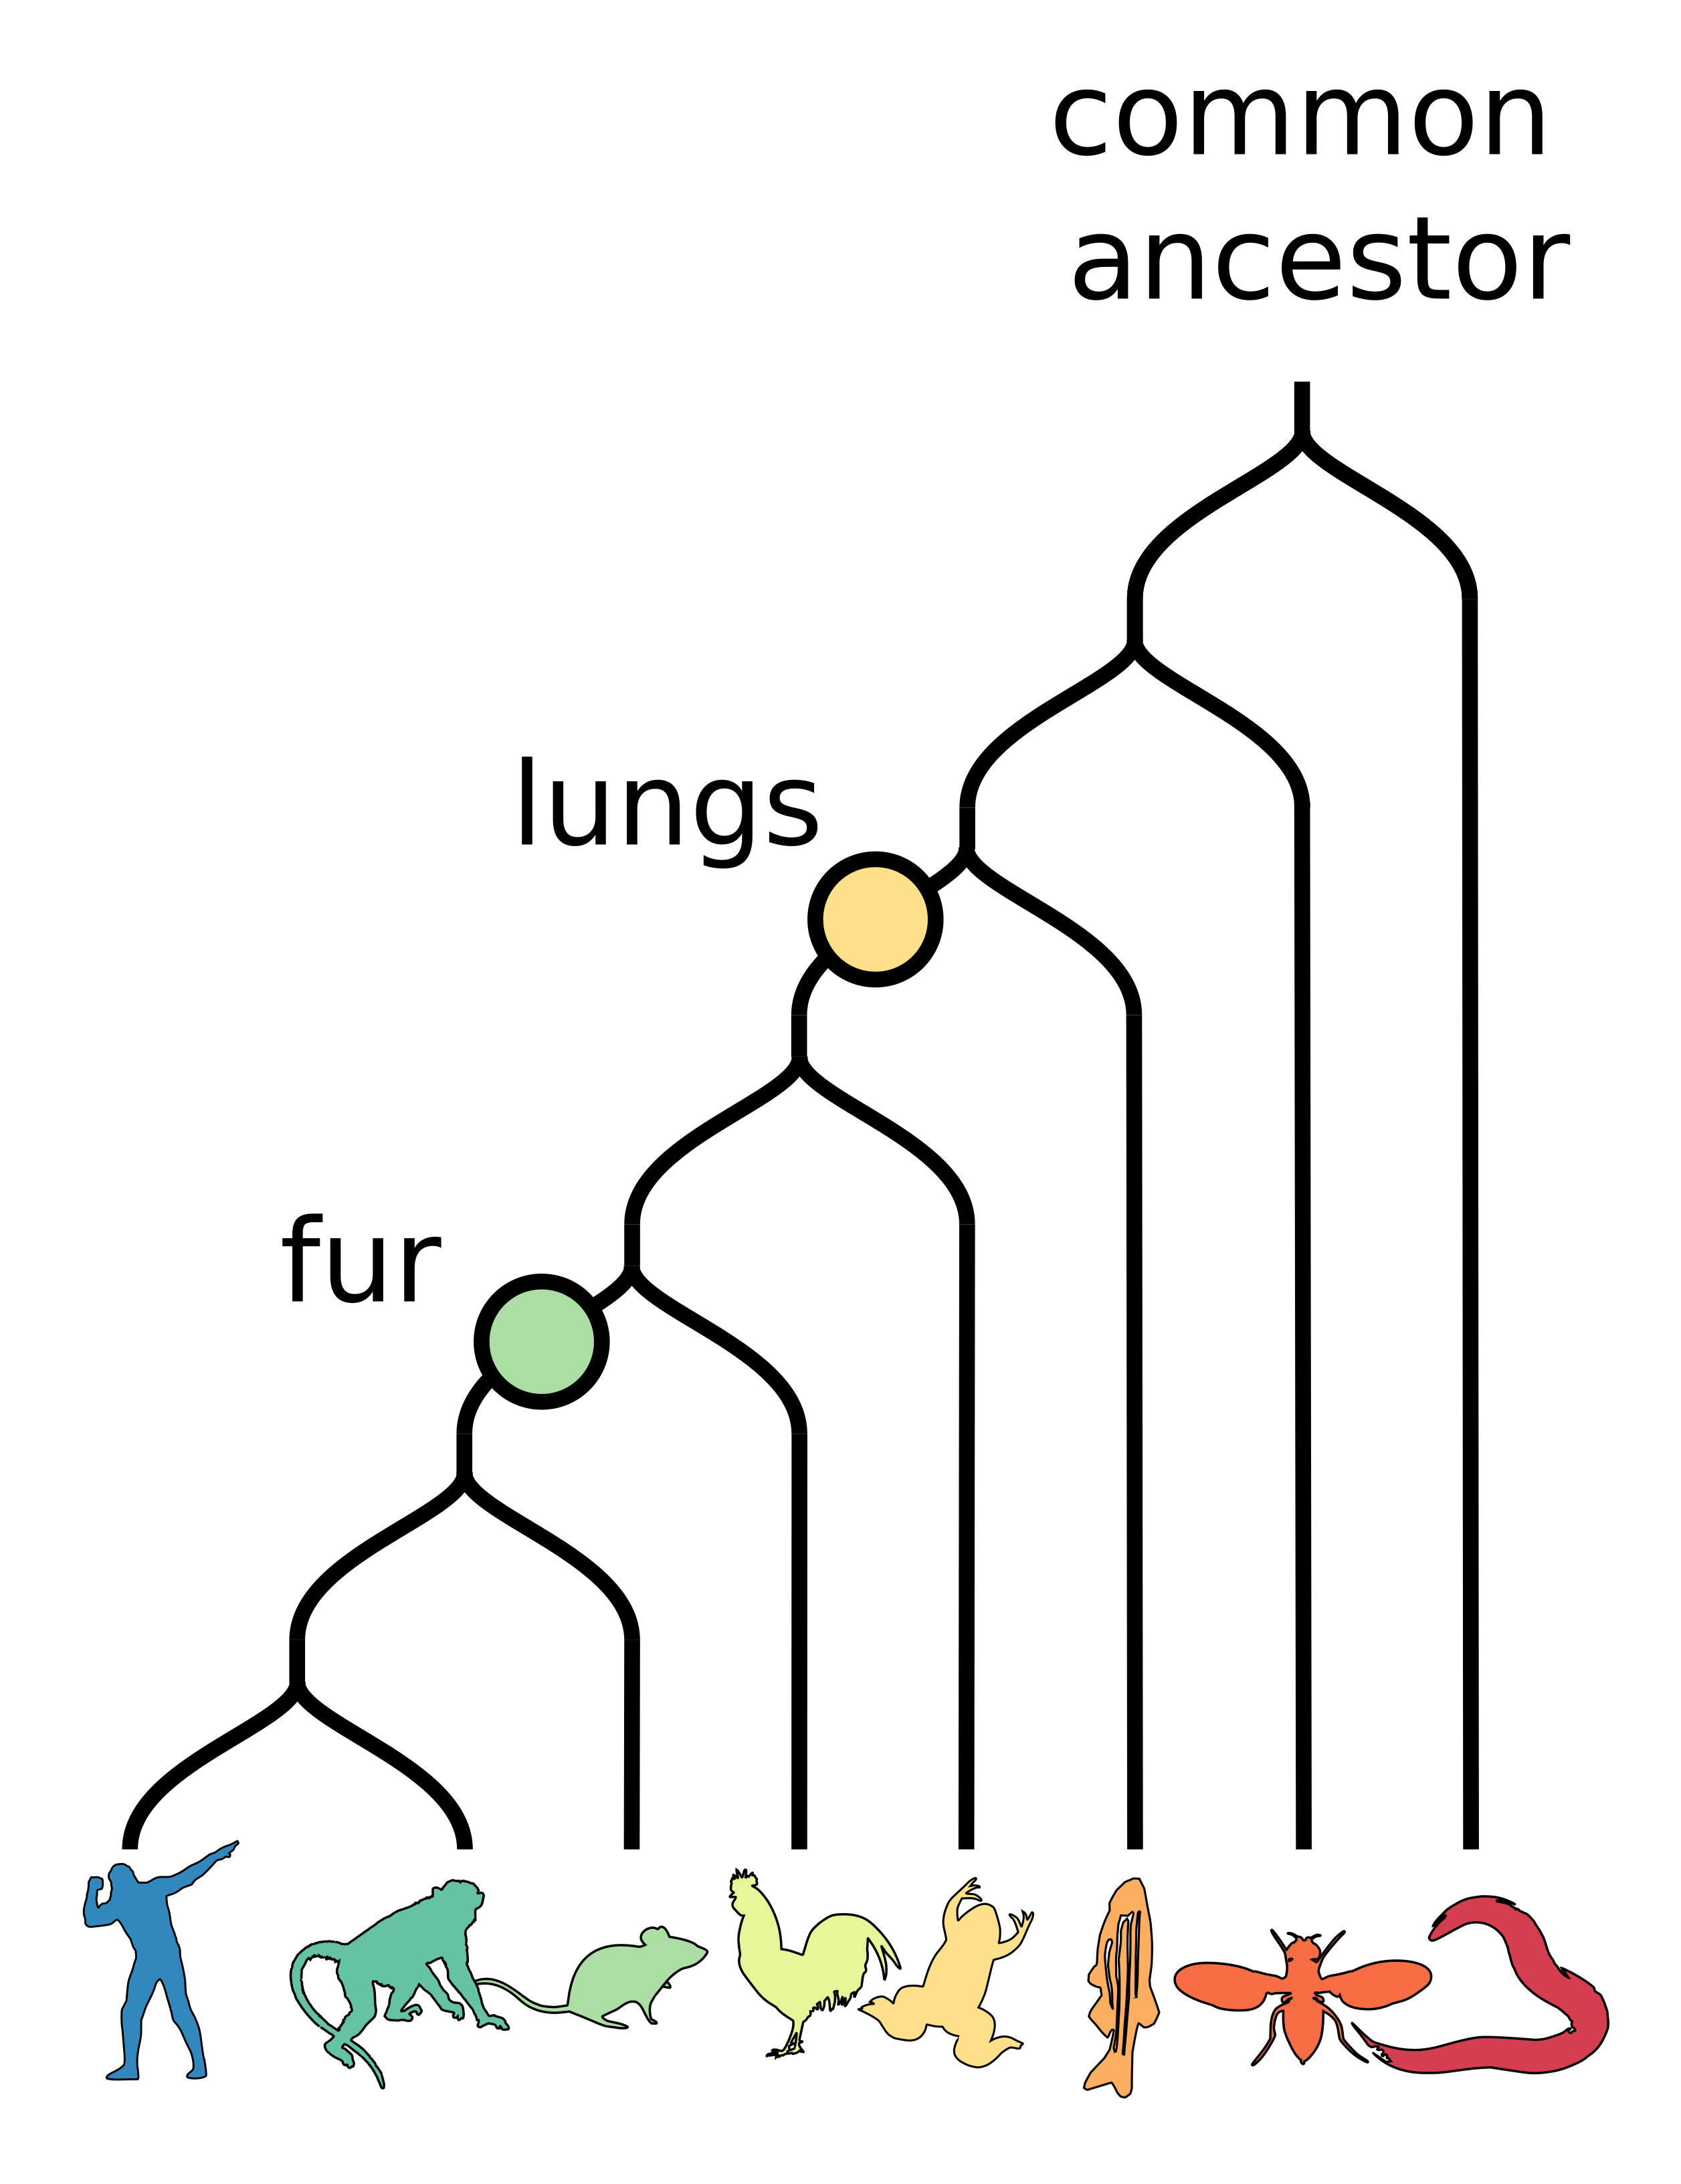
\includegraphics[width=0.5\linewidth]{ch.introduction/imgs/phylogeny.png}
%     \caption{caption}
%     \label{fig:phylogeny}
% \end{figure}

% \subsection{evo-devo gene toolkit}

\subsection{The hourglass model and the phylotypic stage}


% \hvFloat[doublePage,sameHeight]%
%     {figure}%
%     {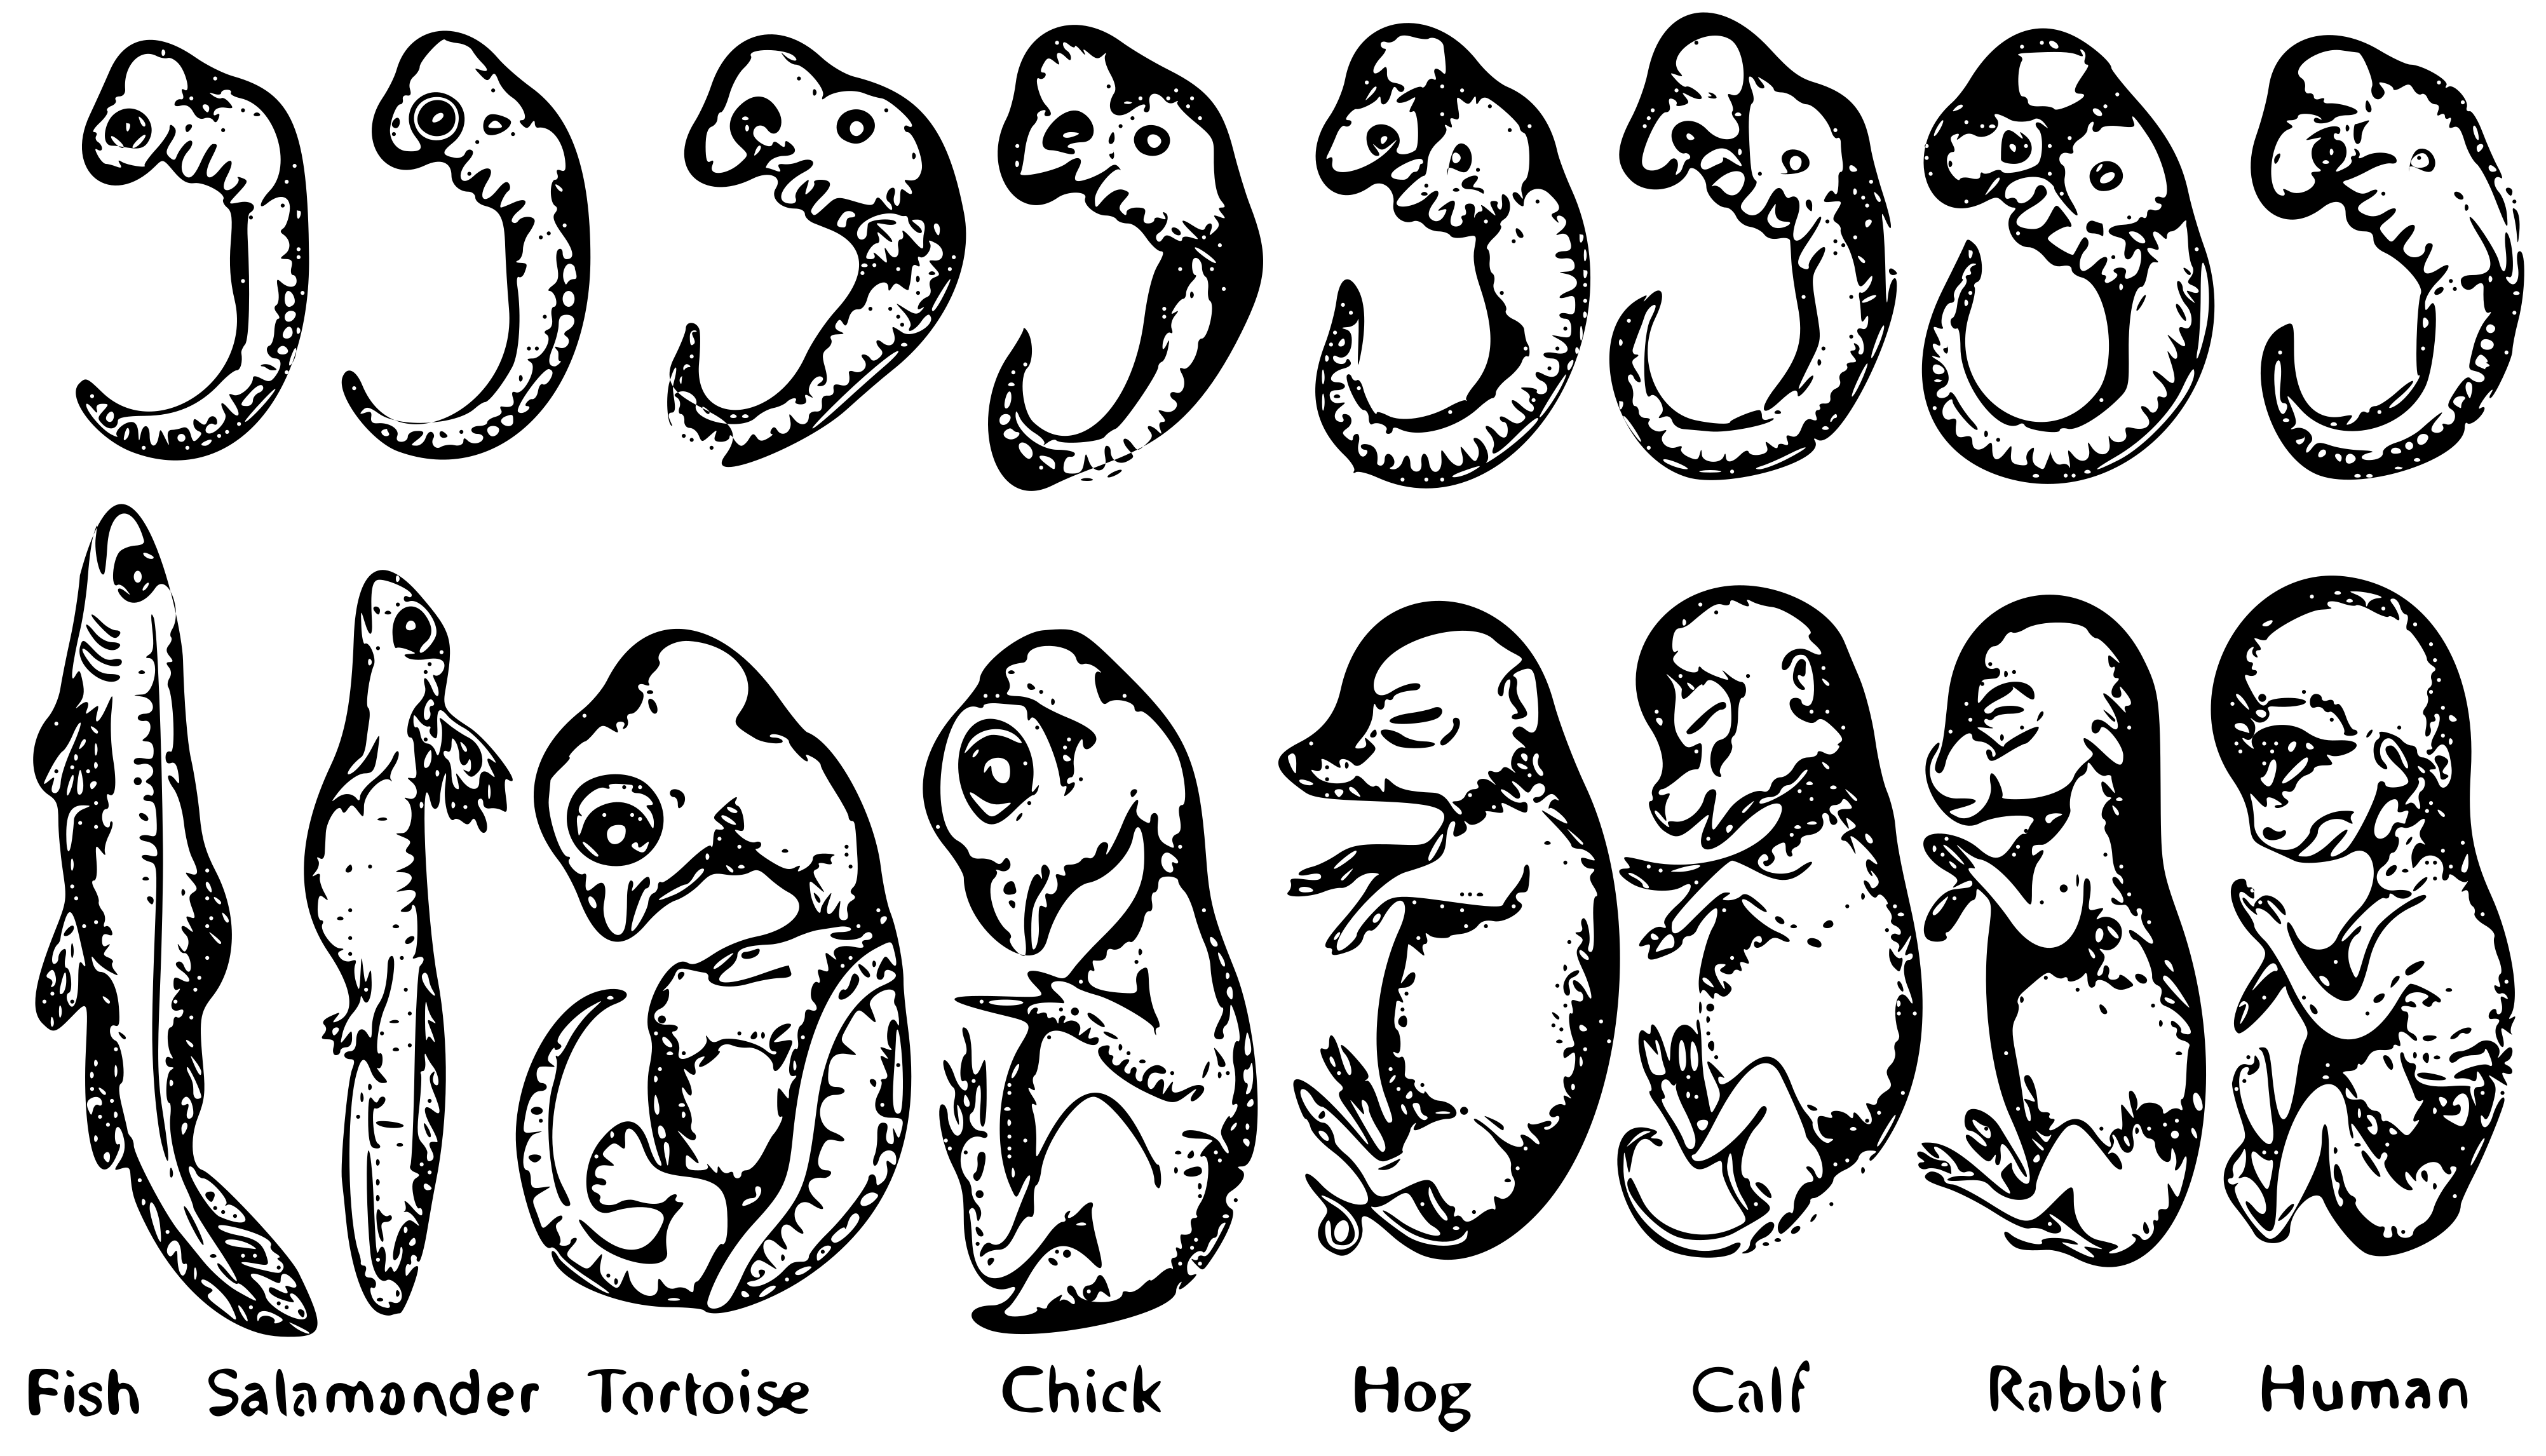
\includegraphics[doublefullPage]{ch.introduction/imgs/haeckel.png}}%
%     [A doublepage image with a caption on the right side of the right part.]%
%     {A caption for a double-sided image that will be placed on the right side of the
%     right-hand part of the illustration. The illustration begins on the left edge of
%     the paper. A short form is used for the LOF.
%     The parameter is \texttt{doublePage}}%
%     {fig:haeckel}


\begin{figure}[H]
    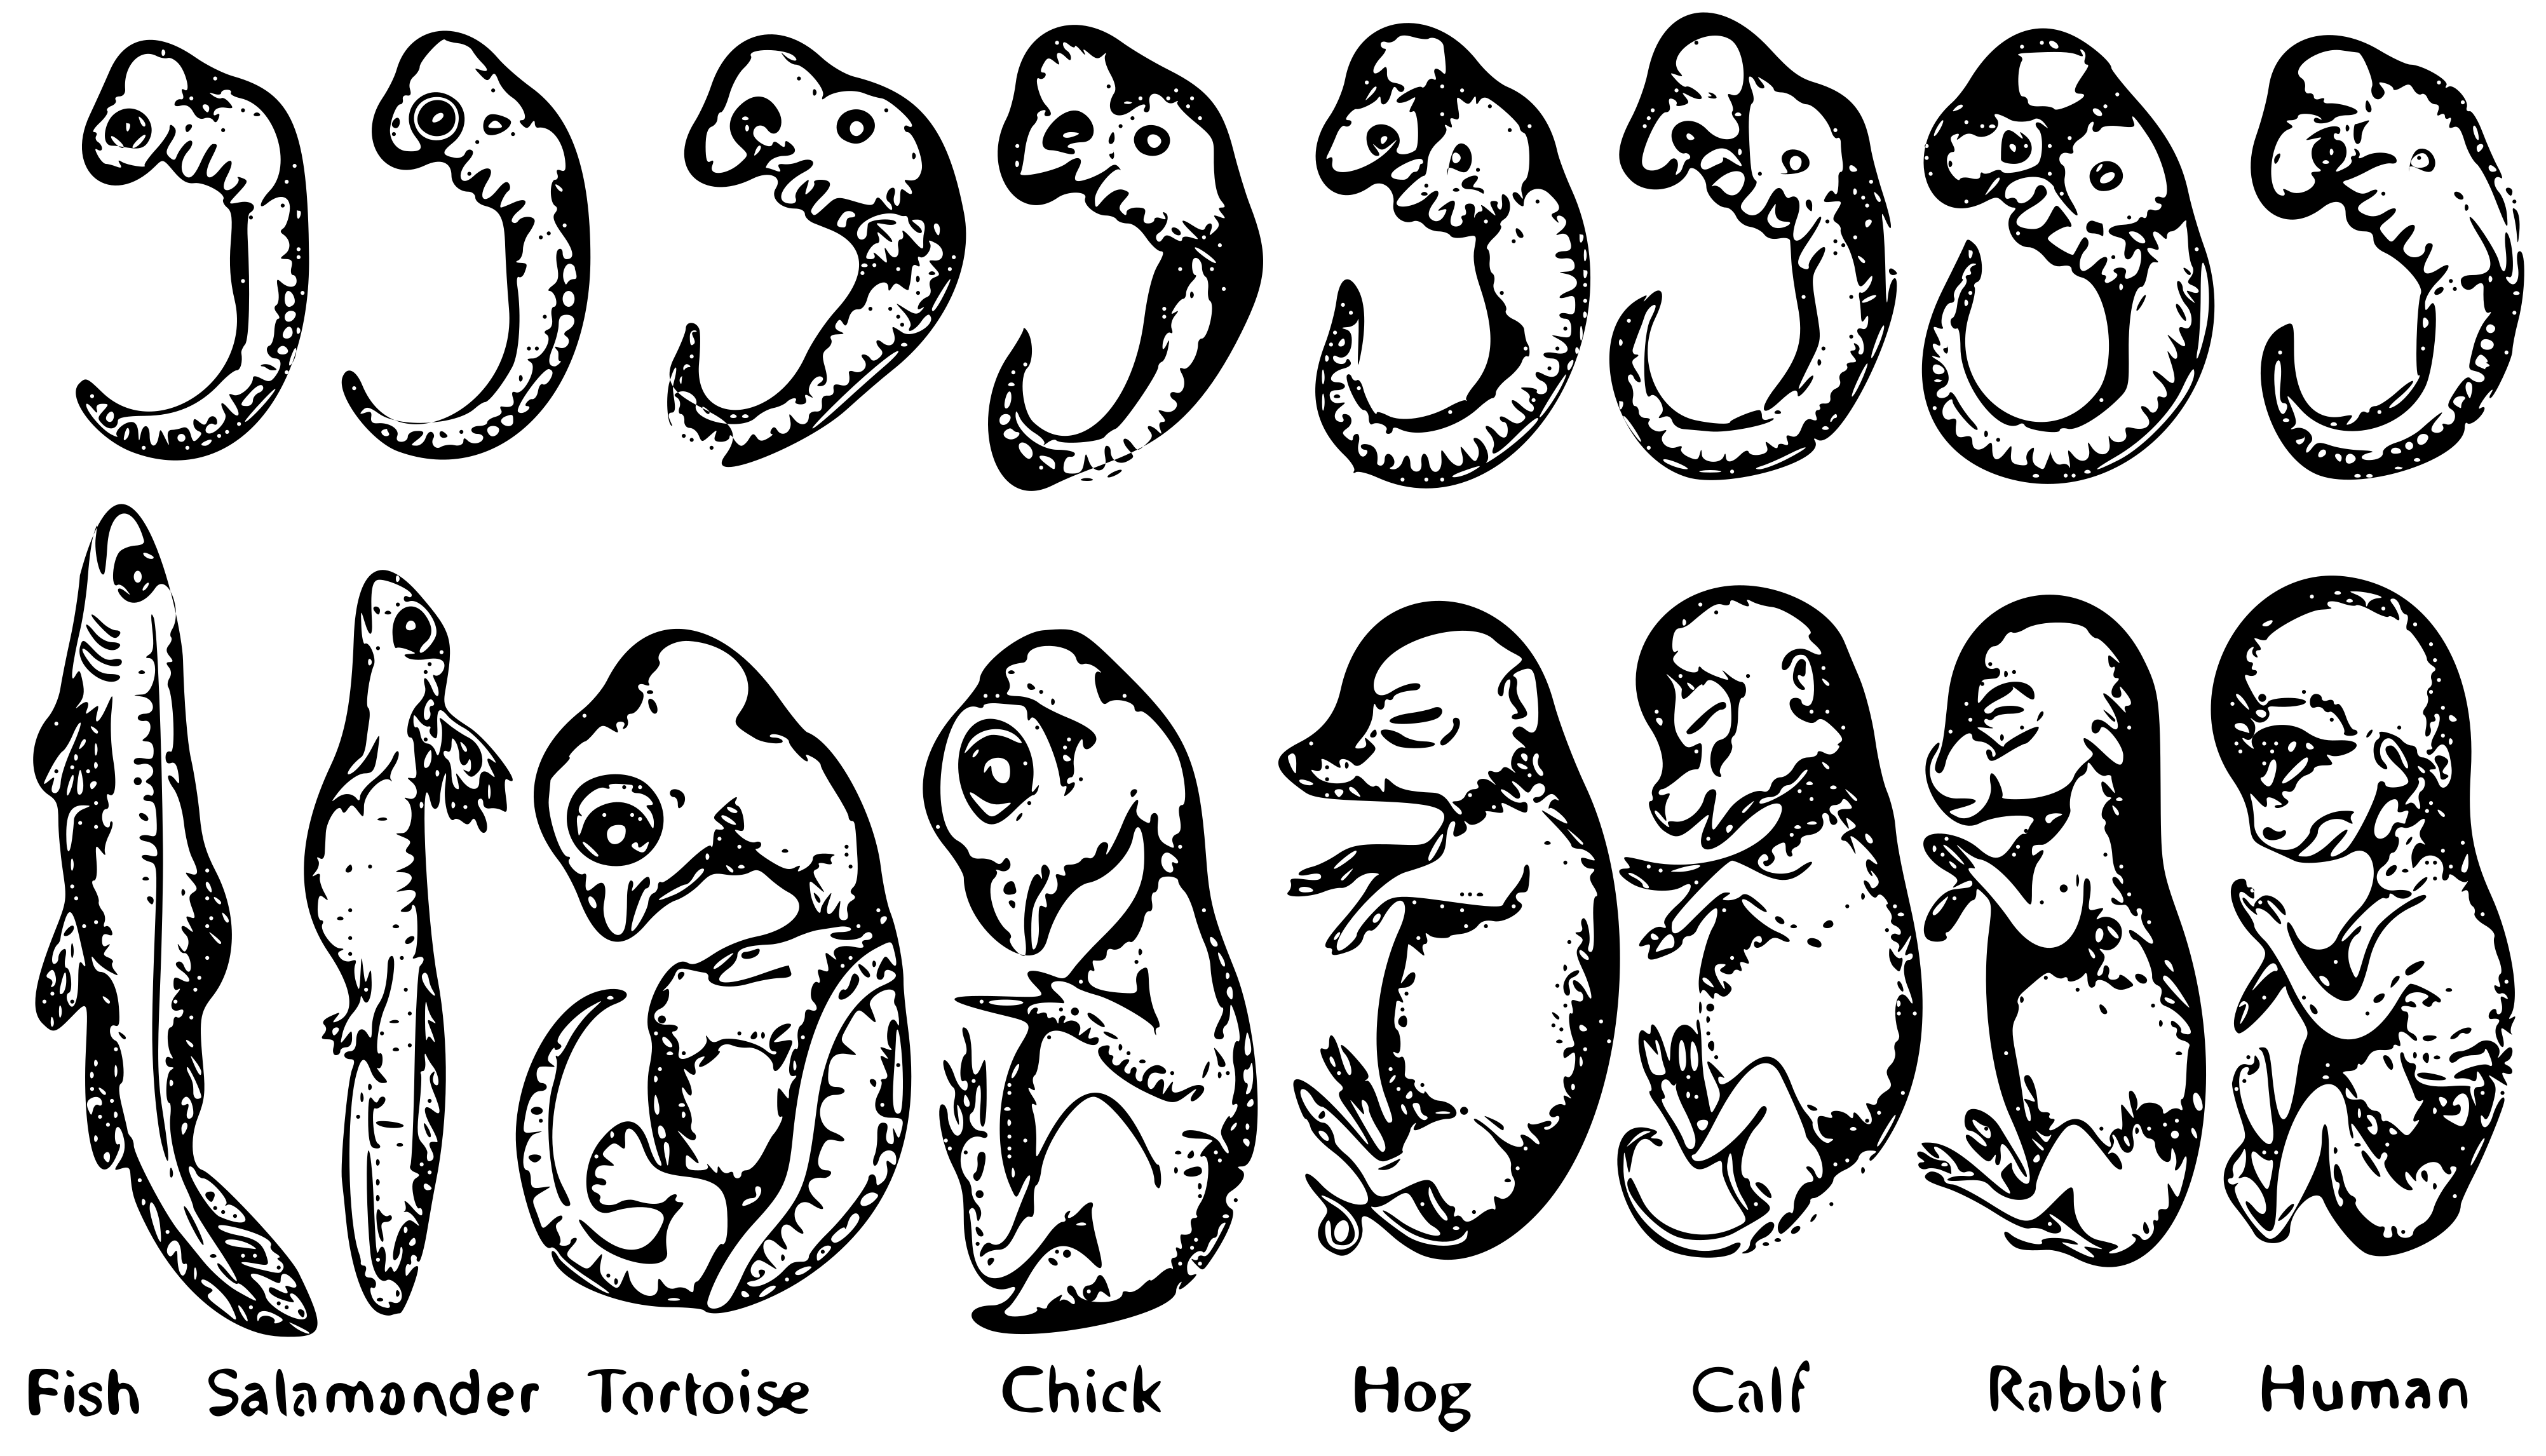
\includegraphics[width=\linewidth]{ch.introduction/imgs/haeckel.png}
    \caption{caption}
    \label{fig:haeckel}
\end{figure}

\begin{figure}[H]
    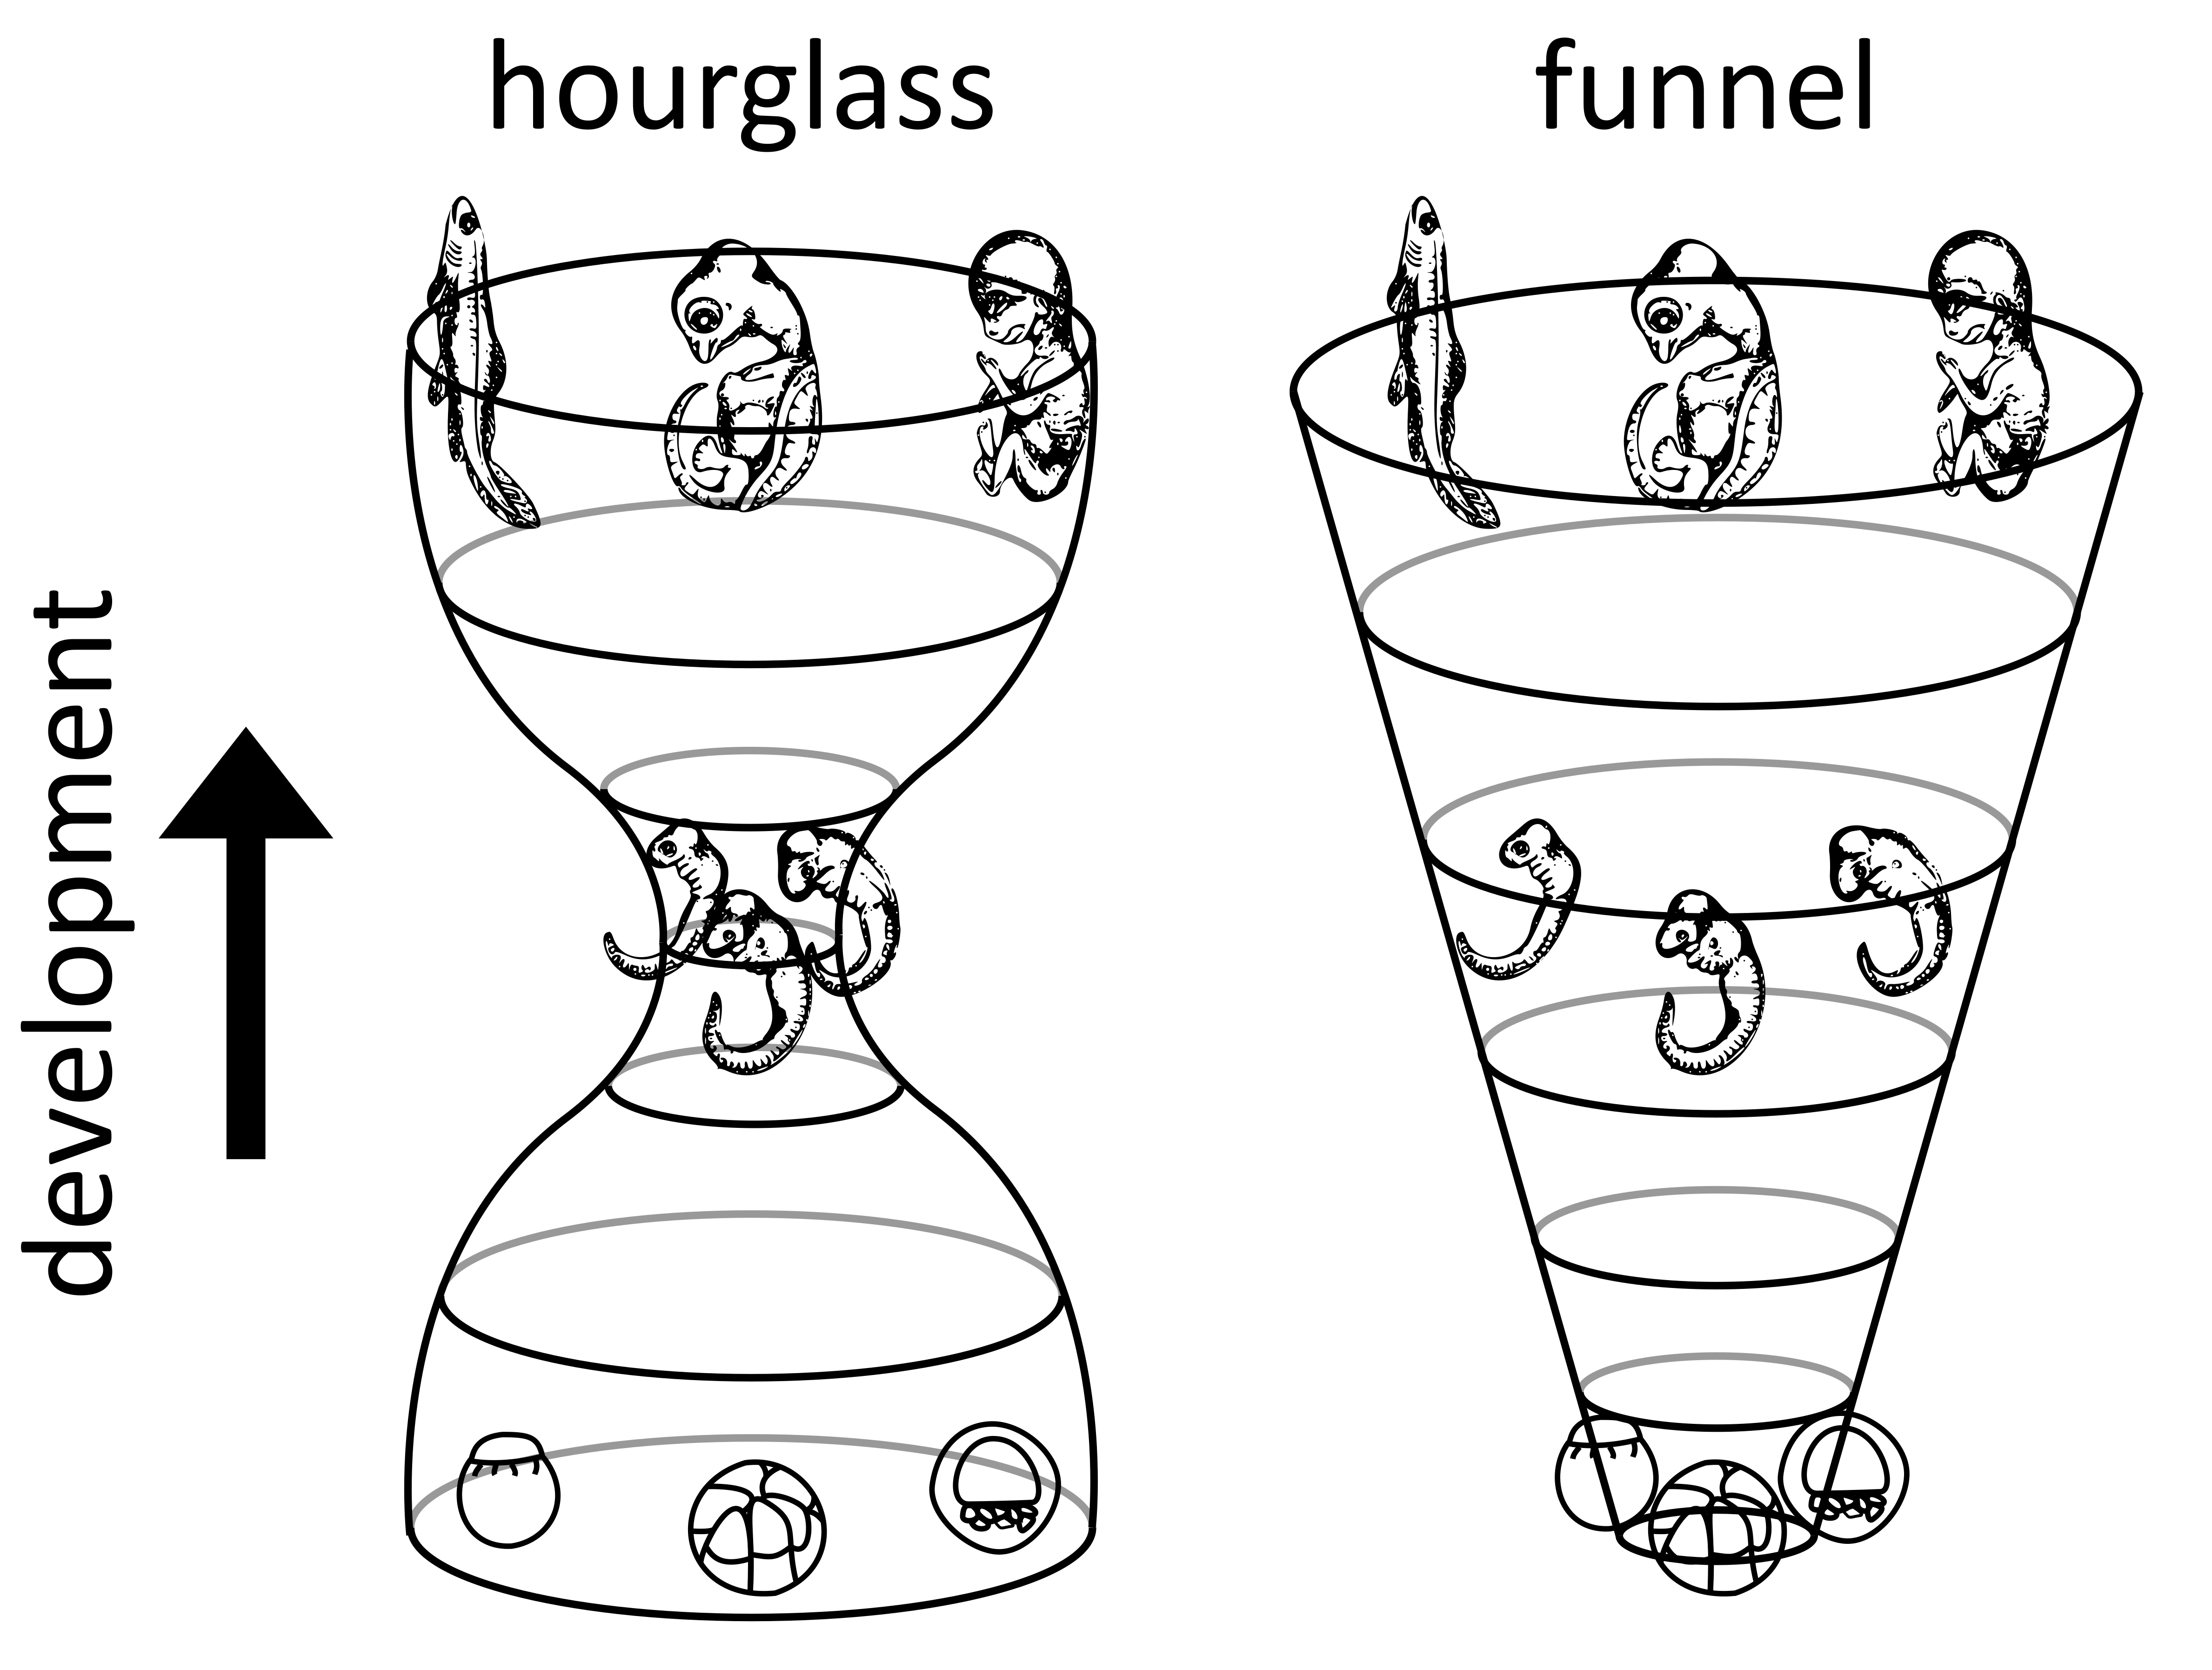
\includegraphics[width=\linewidth]{ch.introduction/imgs/hourglass.png}
    \caption{caption}
    \label{fig:hourglass}
\end{figure}

\section{Computational biology}

The field of computational biology concerns itself with the analysis of the enormous quantities of data that molecular biology produces. In this thesis the analysis of three different sequencing assays 

\begin{figure}[H]
    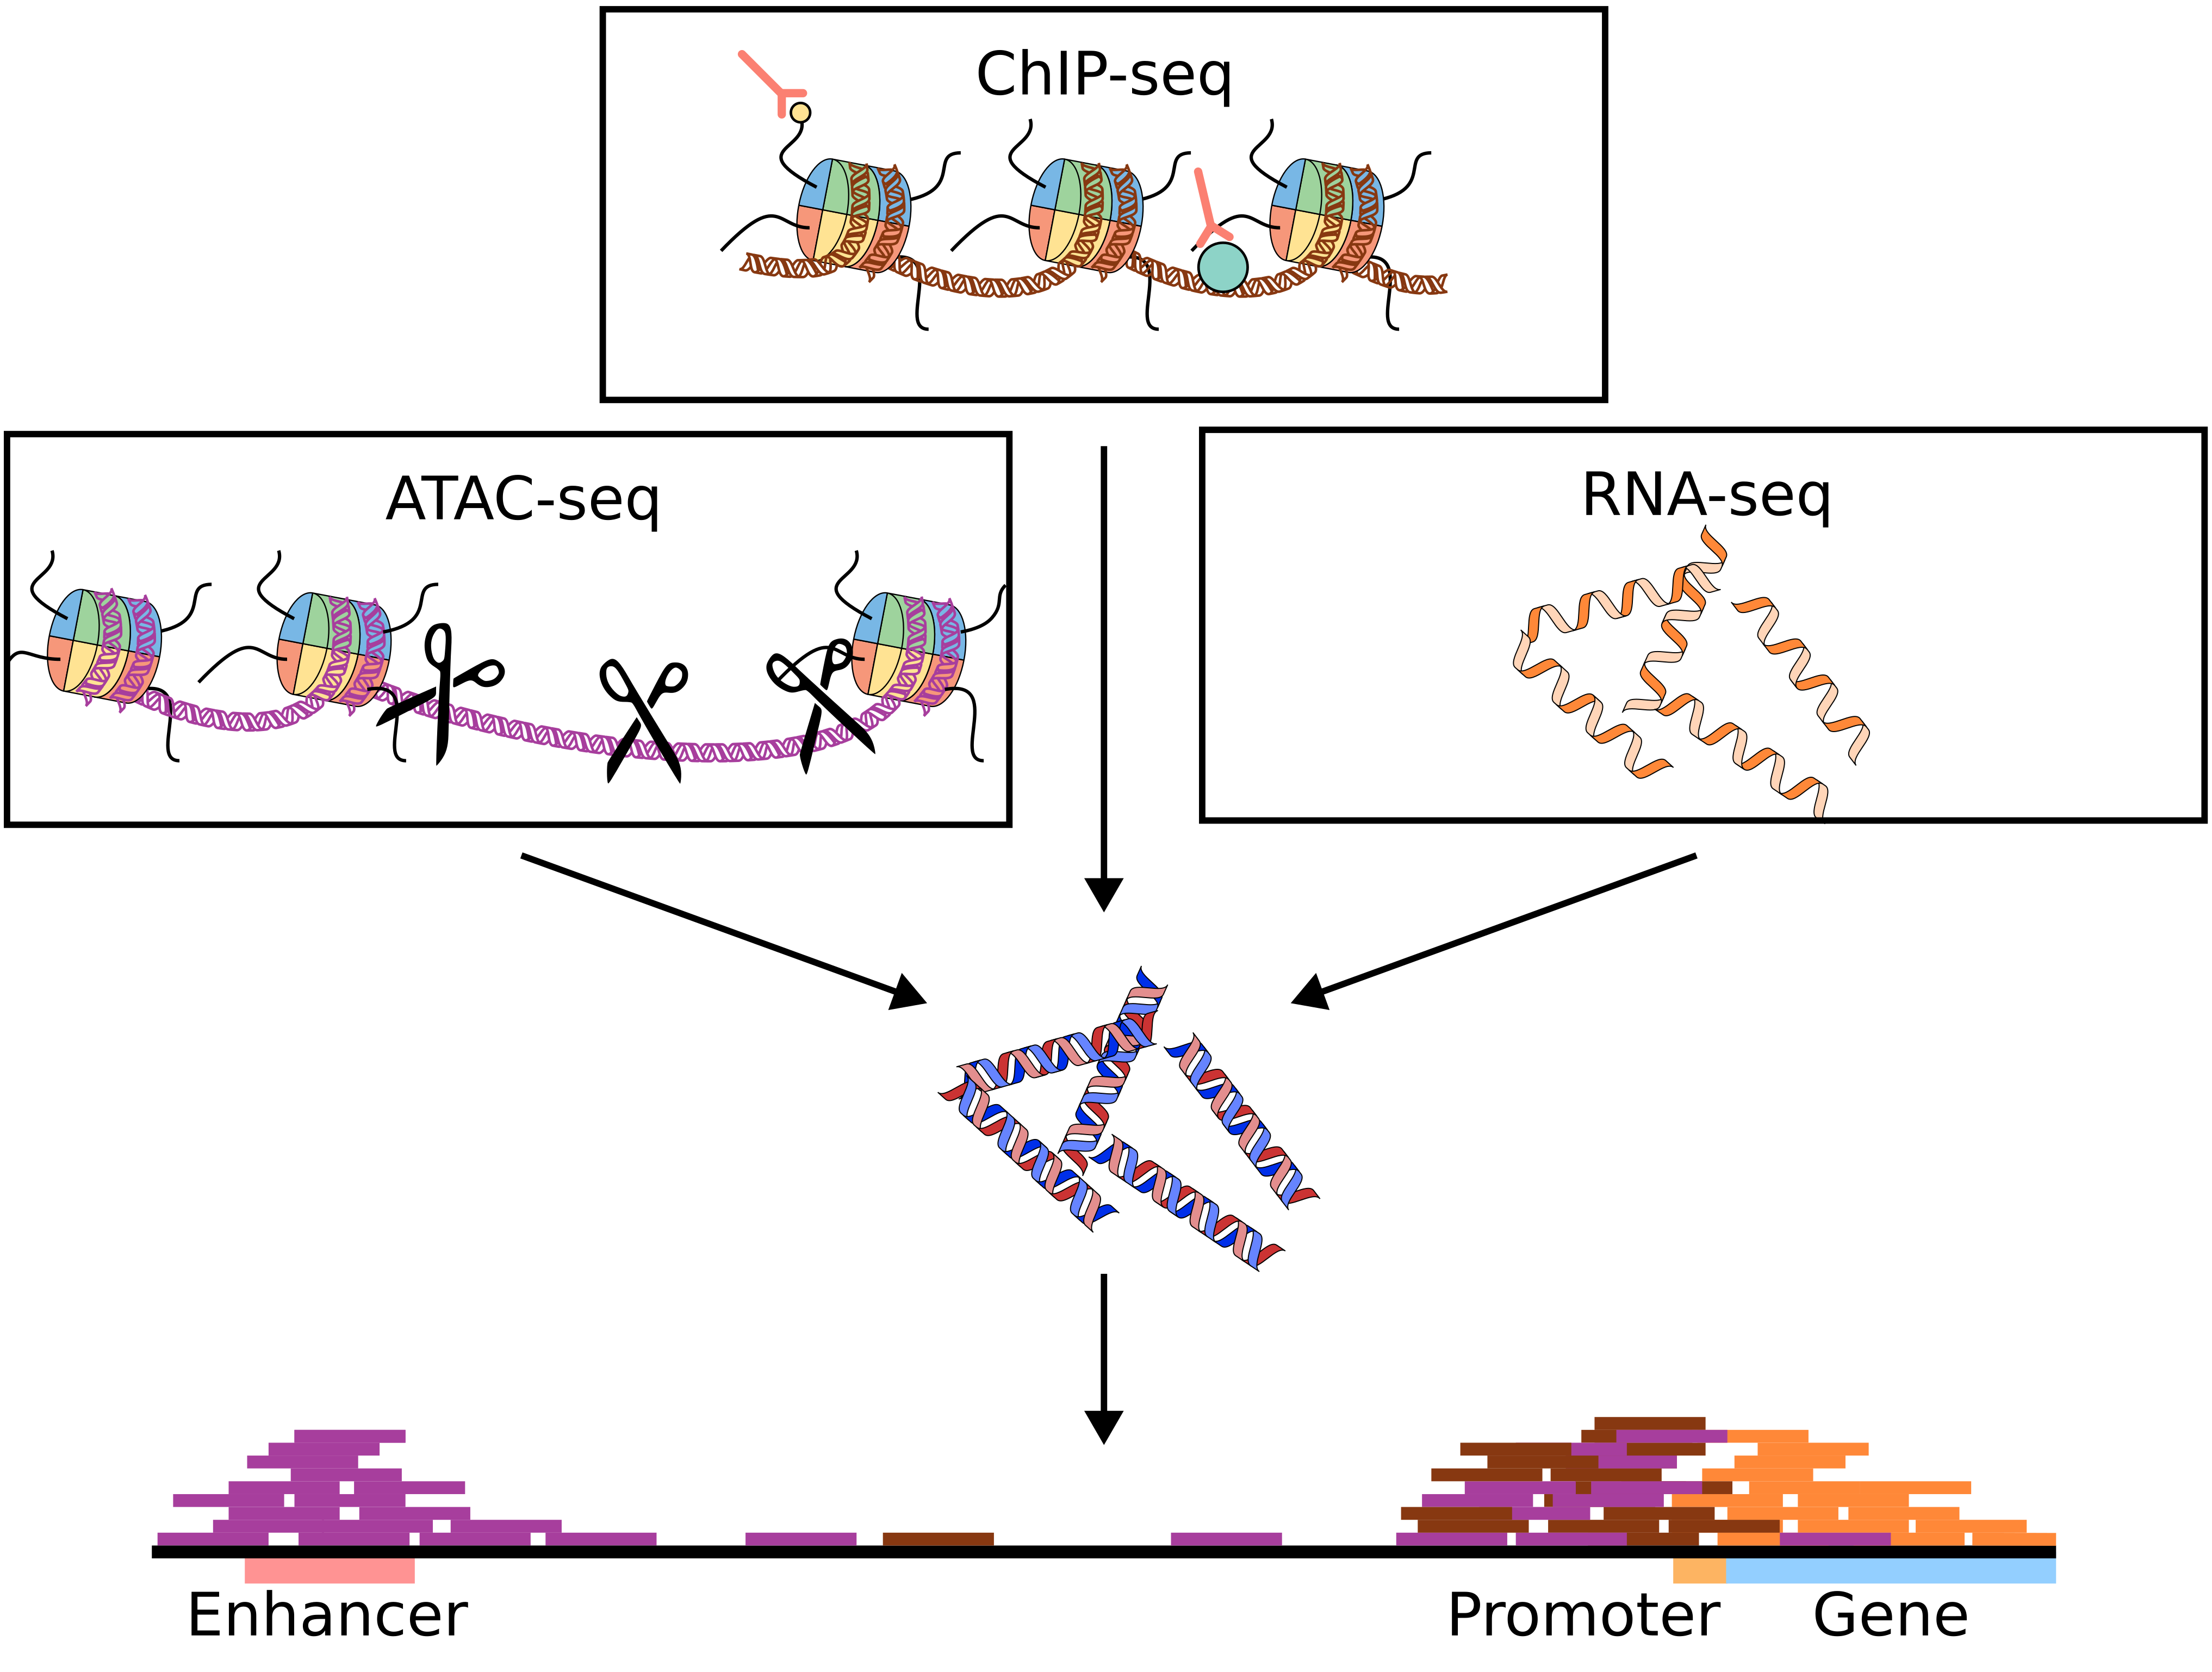
\includegraphics[width=\linewidth]{ch.introduction/imgs/analysis.png}
    \caption{TODO add DNAse}
    \label{fig:analysis}
\end{figure}

\subsection{Single cell}

Whereas originally 

\section{Thesis overview}

The expression and regulation of (embryonic) development is a widely studied topic. It is less common, but still common, to study gene regulation in the context of evolution. Wh

In \textbf{chapter 2} we review the current computational approaches to model and understand gene regulatory networks in development. Current gene regulatory network inference methods perform poorly, and thus a new approach is needed. We highlight three recent developments for gene regulatory network inference which we expect to improve the power of these methods; multi-omics networks, single-cell data, and artificial neural networks. Multi-omics data partially solve the curse of dimensionality by constraining the problem and providing more data. Regular sequencing measures the compounded signal of multiple cell types, single-cell can separate the signal per cell type, so cell-type-specific networks can be made and the data contains purer signal. Artificial neural networks can model more complex gene-gene interactions than the current approaches. By combining these three approaches we expect future gene regulatory network inference methods to predict better networks.

In \textbf{chapter 3} we discuss the implementation of seq2science, a next-generation pre-processing workflow. Seq2science supports some of the most common assays, such as RNA-seq, ChIP-seq, and ATAC-seq, integrates with public databases, and reports an extensive quality control report. Seq2science has been tested on a wide array of different species and genome assemblies, and we show examples of common analyses that seq2science supports out of the box. Seq2science has an extensive user base\cite{Bright_2021,Xu_2020,Wester2021,SantosBarriopedro2021,Heuts2023,Tholen2023,Harlaar2022,LunaVelez2023,Neikes2023,Vierboom2021,Smits2020,Smits2022,Heuts2022,Rother2023}, is downloaded over 40K times through Bioconda, and has more than 120 ``stars'' on GitHub.

In \textbf{chapter 4} we discuss the implementation of Qnorm,  a Python quantile normalization package. Python did not have a quantile normalization package yet, and the implementations on fora about how to do quantile normalization did not resolve ties properly. Qnorm is fast-ish and scales to infinitely large tables as it can swap memory to disk.

In \textbf{chapter 5} we discuss the molecular basis of the phylotypic stage and its related models. We explain how the current definition and analyses of the phylotypic stage are ambiguous, as they do not distinguish within-species effects from between-species effects. For this reason, we propose that any study of the phylotypic stage includes at least a within-species comparison, a within-phylum comparison, and a between-phyla comparison. By applying these comparisons we find important flaws in the interpretation of previous results. We highlight three examples where the within-species pattern is enough to explain the between-species pattern. Moreover, we find that the mid-developmental transition is a statistical artefact. All in all, we question the validity of current approaches to study the phylotypic stage, as they are gross oversimplifications of the biological complexity during development.

In \textbf{chapter 6} 

In \textbf{chapter 7} 
